\documentclass[10pt]{article}
\usepackage[margin=2.2cm]{geometry}
\usepackage{booktabs,longtable,graphicx,array}
\usepackage[hidelinks]{hyperref}
\setlength{\tabcolsep}{4pt}
\newcommand{\stackcell}[1]{\begin{tabular}[t]{@{}l@{}}#1\end{tabular}}
\title{tropical: MaxSubsetSum}
\date{2026-10-25T02:26:04}
\begin{document}
\maketitle

\section{Key results}
This report covers 240 runs (5 seeds; 0 diverged) under frozen hash \texttt{ff2962d32940}.
\paragraph{Where to look.} The headline metric is \texttt{ood\_len\_f1} (higher is better).
\autoref{fig:ood_len_f1} plots it against \texttt{fishr\_lambda}.
\autoref{tab:summary-ood_len_f1} gives every cell's mean with its 95\% bootstrap CI.
\autoref{tab:control-ood_len_f1} compares each level with the control.
\autoref{tab:trend-ood_len_f1} gives the trend.
\autoref{tab:paired-ood_len_f1} gives the paired contrasts.
Its tests take the rank-based path: more than 20\% of values within 0.01 of a bound (0, 1).
Cells are compared within a seed: a seed index fixes the data and the initialization.
Comparisons are marked significant at $p < 0.05$ after the stated correction.

\subsection{\texttt{ood\_len\_f1}}
\begin{figure}[tbp]
\centering
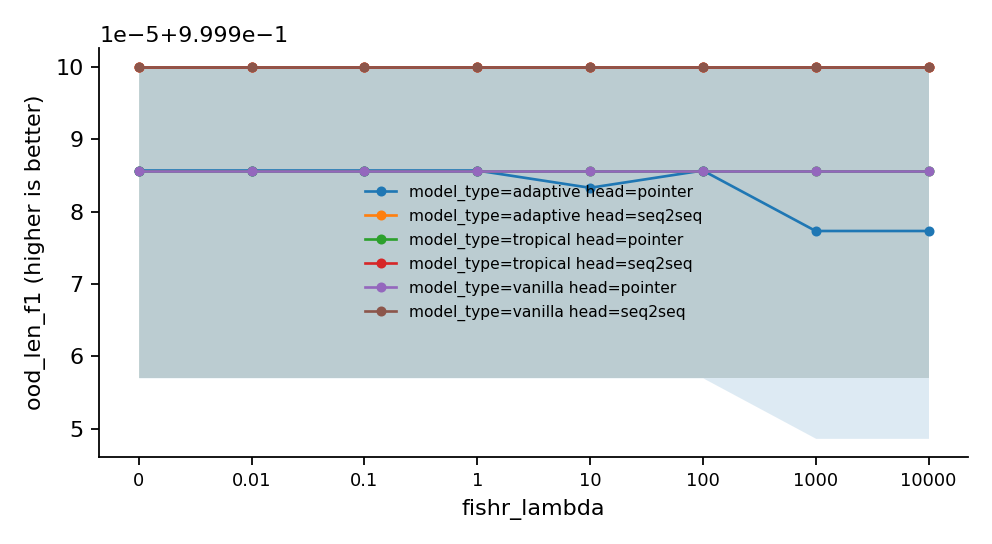
\includegraphics[width=\textwidth]{metric_ood_len_f1.png}
\caption{\texttt{ood\_len\_f1} against \texttt{fishr\_lambda}: the mean over seeds with a 95\% bootstrap CI, one line per combination of the other factors.}
\label{fig:ood_len_f1}
\end{figure}

{\small
\begin{longtable}{lllrlrrr}
\caption{\texttt{ood\_len\_f1} per cell: mean, 95\% bootstrap CI, SD, seeds, diverged runs.}\label{tab:summary-ood_len_f1}\\
\toprule
\texttt{model\_type} & \texttt{head} & \texttt{fishr\_lambda} & mean & 95\% CI & SD & $n$ & div.\\
\midrule
\endhead
adaptive & pointer & 0 & 1 & [1, 1] & $3.20\times10^{-5}$ & 5 & 0\\
adaptive & pointer & 0.01 & 1 & [1, 1] & $3.20\times10^{-5}$ & 5 & 0\\
adaptive & pointer & 0.1 & 1 & [1, 1] & $3.20\times10^{-5}$ & 5 & 0\\
adaptive & pointer & 1 & 1 & [1, 1] & $3.20\times10^{-5}$ & 5 & 0\\
adaptive & pointer & 10 & 1 & [1, 1] & $3.11\times10^{-5}$ & 5 & 0\\
adaptive & pointer & 100 & 1 & [1, 1] & $3.20\times10^{-5}$ & 5 & 0\\
adaptive & pointer & 1000 & 1 & [1, 1] & $3.28\times10^{-5}$ & 5 & 0\\
adaptive & pointer & 1e+04 & 1 & [1, 1] & $3.28\times10^{-5}$ & 5 & 0\\
adaptive & seq2seq & 0 & 1 & [1, 1] & 0 & 5 & 0\\
adaptive & seq2seq & 0.01 & 1 & [1, 1] & 0 & 5 & 0\\
adaptive & seq2seq & 0.1 & 1 & [1, 1] & 0 & 5 & 0\\
adaptive & seq2seq & 1 & 1 & [1, 1] & 0 & 5 & 0\\
adaptive & seq2seq & 10 & 1 & [1, 1] & 0 & 5 & 0\\
adaptive & seq2seq & 100 & 1 & [1, 1] & 0 & 5 & 0\\
adaptive & seq2seq & 1000 & 1 & [1, 1] & 0 & 5 & 0\\
adaptive & seq2seq & 1e+04 & 1 & [1, 1] & 0 & 5 & 0\\
tropical & pointer & 0 & 1 & [1, 1] & $3.20\times10^{-5}$ & 5 & 0\\
tropical & pointer & 0.01 & 1 & [1, 1] & $3.20\times10^{-5}$ & 5 & 0\\
tropical & pointer & 0.1 & 1 & [1, 1] & $3.20\times10^{-5}$ & 5 & 0\\
tropical & pointer & 1 & 1 & [1, 1] & $3.20\times10^{-5}$ & 5 & 0\\
tropical & pointer & 10 & 1 & [1, 1] & $3.20\times10^{-5}$ & 5 & 0\\
tropical & pointer & 100 & 1 & [1, 1] & $3.20\times10^{-5}$ & 5 & 0\\
tropical & pointer & 1000 & 1 & [1, 1] & $3.20\times10^{-5}$ & 5 & 0\\
tropical & pointer & 1e+04 & 1 & [1, 1] & $3.20\times10^{-5}$ & 5 & 0\\
tropical & seq2seq & 0 & 1 & [1, 1] & 0 & 5 & 0\\
tropical & seq2seq & 0.01 & 1 & [1, 1] & 0 & 5 & 0\\
tropical & seq2seq & 0.1 & 1 & [1, 1] & 0 & 5 & 0\\
tropical & seq2seq & 1 & 1 & [1, 1] & 0 & 5 & 0\\
tropical & seq2seq & 10 & 1 & [1, 1] & 0 & 5 & 0\\
tropical & seq2seq & 100 & 1 & [1, 1] & 0 & 5 & 0\\
tropical & seq2seq & 1000 & 1 & [1, 1] & 0 & 5 & 0\\
tropical & seq2seq & 1e+04 & 1 & [1, 1] & 0 & 5 & 0\\
vanilla & pointer & 0 & 1 & [1, 1] & $3.20\times10^{-5}$ & 5 & 0\\
vanilla & pointer & 0.01 & 1 & [1, 1] & $3.20\times10^{-5}$ & 5 & 0\\
vanilla & pointer & 0.1 & 1 & [1, 1] & $3.20\times10^{-5}$ & 5 & 0\\
vanilla & pointer & 1 & 1 & [1, 1] & $3.20\times10^{-5}$ & 5 & 0\\
vanilla & pointer & 10 & 1 & [1, 1] & $3.20\times10^{-5}$ & 5 & 0\\
vanilla & pointer & 100 & 1 & [1, 1] & $3.20\times10^{-5}$ & 5 & 0\\
vanilla & pointer & 1000 & 1 & [1, 1] & $3.20\times10^{-5}$ & 5 & 0\\
vanilla & pointer & 1e+04 & 1 & [1, 1] & $3.20\times10^{-5}$ & 5 & 0\\
vanilla & seq2seq & 0 & 1 & [1, 1] & 0 & 5 & 0\\
vanilla & seq2seq & 0.01 & 1 & [1, 1] & 0 & 5 & 0\\
vanilla & seq2seq & 0.1 & 1 & [1, 1] & 0 & 5 & 0\\
vanilla & seq2seq & 1 & 1 & [1, 1] & 0 & 5 & 0\\
vanilla & seq2seq & 10 & 1 & [1, 1] & 0 & 5 & 0\\
vanilla & seq2seq & 100 & 1 & [1, 1] & 0 & 5 & 0\\
vanilla & seq2seq & 1000 & 1 & [1, 1] & 0 & 5 & 0\\
vanilla & seq2seq & 1e+04 & 1 & [1, 1] & 0 & 5 & 0\\
\bottomrule
\end{longtable}
}

{\small
\begin{longtable}{lllrrrl}
\caption{\texttt{ood\_len\_f1}: each level of \texttt{fishr\_lambda} against its control (0), within each combination of the other factors. rank: Wilcoxon signed-rank by seed, Holm.}\label{tab:control-ood_len_f1}\\
\toprule
\texttt{model\_type} & \texttt{head} & \texttt{fishr\_lambda} & difference & 95\% CI & $p$ & \\
\midrule
\endhead
adaptive & pointer & 0.01 & 0 & [0, 0] & -- & \\
adaptive & pointer & 0.1 & 0 & [0, 0] & -- & \\
adaptive & pointer & 1 & 0 & [0, 0] & -- & \\
adaptive & pointer & 10 & 0 & [$-7.16\times10^{-6}$, 0] & 1.0000 & \\
adaptive & pointer & 100 & 0 & [0, 0] & -- & \\
adaptive & pointer & 1000 & 0 & [$-2.51\times10^{-5}$, 0] & 1.0000 & \\
adaptive & pointer & 1e+04 & 0 & [$-2.51\times10^{-5}$, 0] & 1.0000 & \\
adaptive & seq2seq & 0.01 & 0 & [0, 0] & -- & \\
adaptive & seq2seq & 0.1 & 0 & [0, 0] & -- & \\
adaptive & seq2seq & 1 & 0 & [0, 0] & -- & \\
adaptive & seq2seq & 10 & 0 & [0, 0] & -- & \\
adaptive & seq2seq & 100 & 0 & [0, 0] & -- & \\
adaptive & seq2seq & 1000 & 0 & [0, 0] & -- & \\
adaptive & seq2seq & 1e+04 & 0 & [0, 0] & -- & \\
tropical & pointer & 0.01 & 0 & [0, 0] & -- & \\
tropical & pointer & 0.1 & 0 & [0, 0] & -- & \\
tropical & pointer & 1 & 0 & [0, 0] & -- & \\
tropical & pointer & 10 & 0 & [0, 0] & -- & \\
tropical & pointer & 100 & 0 & [0, 0] & -- & \\
tropical & pointer & 1000 & 0 & [0, 0] & -- & \\
tropical & pointer & 1e+04 & 0 & [0, 0] & -- & \\
tropical & seq2seq & 0.01 & 0 & [0, 0] & -- & \\
tropical & seq2seq & 0.1 & 0 & [0, 0] & -- & \\
tropical & seq2seq & 1 & 0 & [0, 0] & -- & \\
tropical & seq2seq & 10 & 0 & [0, 0] & -- & \\
tropical & seq2seq & 100 & 0 & [0, 0] & -- & \\
tropical & seq2seq & 1000 & 0 & [0, 0] & -- & \\
tropical & seq2seq & 1e+04 & 0 & [0, 0] & -- & \\
vanilla & pointer & 0.01 & 0 & [0, 0] & -- & \\
vanilla & pointer & 0.1 & 0 & [0, 0] & -- & \\
vanilla & pointer & 1 & 0 & [0, 0] & -- & \\
vanilla & pointer & 10 & 0 & [0, 0] & -- & \\
vanilla & pointer & 100 & 0 & [0, 0] & -- & \\
vanilla & pointer & 1000 & 0 & [0, 0] & -- & \\
vanilla & pointer & 1e+04 & 0 & [0, 0] & -- & \\
vanilla & seq2seq & 0.01 & 0 & [0, 0] & -- & \\
vanilla & seq2seq & 0.1 & 0 & [0, 0] & -- & \\
vanilla & seq2seq & 1 & 0 & [0, 0] & -- & \\
vanilla & seq2seq & 10 & 0 & [0, 0] & -- & \\
vanilla & seq2seq & 100 & 0 & [0, 0] & -- & \\
vanilla & seq2seq & 1000 & 0 & [0, 0] & -- & \\
vanilla & seq2seq & 1e+04 & 0 & [0, 0] & -- & \\
\bottomrule
\end{longtable}
}

{\small
\begin{longtable}{llrrrrr}
\caption{\texttt{ood\_len\_f1} against log10 \texttt{fishr\_lambda}: rank: Spearman rho, seed-bootstrap CI, with the Jonckheere--Terpstra ordered-trend $\tau$ and $p$.}\label{tab:trend-ood_len_f1}\\
\toprule
\texttt{model\_type} & \texttt{head} & estimate & 95\% CI & $p$ & JT $\tau$ & JT $p$\\
\midrule
\endhead
adaptive & pointer & -0.1294 & [-0.527, 0] & 0.4587 & -0.08 & 0.4603\\
adaptive & seq2seq & -- & [--, --] & -- & -- & --\\
tropical & pointer & 0 & [0, 0] & 1.0000 & 0 & 1.0000\\
tropical & seq2seq & -- & [--, --] & -- & -- & --\\
vanilla & pointer & 0 & [0, 0] & 1.0000 & 0 & 1.0000\\
vanilla & seq2seq & -- & [--, --] & -- & -- & --\\
\bottomrule
\end{longtable}
}

{\small
\begin{longtable}{lrrrl}
\caption{\texttt{ood\_len\_f1}: paired contrasts by seed, Holm-corrected across the cells. rank: Wilcoxon signed-rank by seed, Holm.}\label{tab:paired-ood_len_f1}\\
\toprule
contrast (within) & difference & 95\% CI & $p$ & \\
\midrule
\endhead
\stackcell{model\_type: tropical - vanilla\\\footnotesize head=pointer fishr\_lambda=0 } & 0 & [--, --] & -- & \\
\stackcell{model\_type: tropical - vanilla\\\footnotesize head=pointer fishr\_lambda=0.01 } & 0 & [--, --] & -- & \\
\stackcell{model\_type: tropical - vanilla\\\footnotesize head=pointer fishr\_lambda=0.1 } & 0 & [--, --] & -- & \\
\stackcell{model\_type: tropical - vanilla\\\footnotesize head=pointer fishr\_lambda=1 } & 0 & [--, --] & -- & \\
\stackcell{model\_type: tropical - vanilla\\\footnotesize head=pointer fishr\_lambda=10 } & 0 & [--, --] & -- & \\
\stackcell{model\_type: tropical - vanilla\\\footnotesize head=pointer fishr\_lambda=100 } & 0 & [--, --] & -- & \\
\stackcell{model\_type: tropical - vanilla\\\footnotesize head=pointer fishr\_lambda=1000 } & 0 & [--, --] & -- & \\
\stackcell{model\_type: tropical - vanilla\\\footnotesize head=pointer fishr\_lambda=1e+04 } & 0 & [--, --] & -- & \\
\stackcell{model\_type: tropical - vanilla\\\footnotesize head=seq2seq fishr\_lambda=0 } & 0 & [--, --] & -- & \\
\stackcell{model\_type: tropical - vanilla\\\footnotesize head=seq2seq fishr\_lambda=0.01 } & 0 & [--, --] & -- & \\
\stackcell{model\_type: tropical - vanilla\\\footnotesize head=seq2seq fishr\_lambda=0.1 } & 0 & [--, --] & -- & \\
\stackcell{model\_type: tropical - vanilla\\\footnotesize head=seq2seq fishr\_lambda=1 } & 0 & [--, --] & -- & \\
\stackcell{model\_type: tropical - vanilla\\\footnotesize head=seq2seq fishr\_lambda=10 } & 0 & [--, --] & -- & \\
\stackcell{model\_type: tropical - vanilla\\\footnotesize head=seq2seq fishr\_lambda=100 } & 0 & [--, --] & -- & \\
\stackcell{model\_type: tropical - vanilla\\\footnotesize head=seq2seq fishr\_lambda=1000 } & 0 & [--, --] & -- & \\
\stackcell{model\_type: tropical - vanilla\\\footnotesize head=seq2seq fishr\_lambda=1e+04 } & 0 & [--, --] & -- & \\
\stackcell{model\_type: adaptive - vanilla\\\footnotesize head=pointer fishr\_lambda=0 } & 0 & [--, --] & -- & \\
\stackcell{model\_type: adaptive - vanilla\\\footnotesize head=pointer fishr\_lambda=0.01 } & 0 & [--, --] & -- & \\
\stackcell{model\_type: adaptive - vanilla\\\footnotesize head=pointer fishr\_lambda=0.1 } & 0 & [--, --] & -- & \\
\stackcell{model\_type: adaptive - vanilla\\\footnotesize head=pointer fishr\_lambda=1 } & 0 & [--, --] & -- & \\
\stackcell{model\_type: adaptive - vanilla\\\footnotesize head=pointer fishr\_lambda=10 } & $-2.387\times10^{-6}$ & [$-9.01\times10^{-6}$, $4.24\times10^{-6}$] & 1.0000 & \\
\stackcell{model\_type: adaptive - vanilla\\\footnotesize head=pointer fishr\_lambda=100 } & 0 & [--, --] & -- & \\
\stackcell{model\_type: adaptive - vanilla\\\footnotesize head=pointer fishr\_lambda=1000 } & $-8.354\times10^{-6}$ & [$-3.15\times10^{-5}$, $1.48\times10^{-5}$] & 1.0000 & \\
\stackcell{model\_type: adaptive - vanilla\\\footnotesize head=pointer fishr\_lambda=1e+04 } & $-8.354\times10^{-6}$ & [$-3.15\times10^{-5}$, $1.48\times10^{-5}$] & 1.0000 & \\
\stackcell{model\_type: adaptive - vanilla\\\footnotesize head=seq2seq fishr\_lambda=0 } & 0 & [--, --] & -- & \\
\stackcell{model\_type: adaptive - vanilla\\\footnotesize head=seq2seq fishr\_lambda=0.01 } & 0 & [--, --] & -- & \\
\stackcell{model\_type: adaptive - vanilla\\\footnotesize head=seq2seq fishr\_lambda=0.1 } & 0 & [--, --] & -- & \\
\stackcell{model\_type: adaptive - vanilla\\\footnotesize head=seq2seq fishr\_lambda=1 } & 0 & [--, --] & -- & \\
\stackcell{model\_type: adaptive - vanilla\\\footnotesize head=seq2seq fishr\_lambda=10 } & 0 & [--, --] & -- & \\
\stackcell{model\_type: adaptive - vanilla\\\footnotesize head=seq2seq fishr\_lambda=100 } & 0 & [--, --] & -- & \\
\stackcell{model\_type: adaptive - vanilla\\\footnotesize head=seq2seq fishr\_lambda=1000 } & 0 & [--, --] & -- & \\
\stackcell{model\_type: adaptive - vanilla\\\footnotesize head=seq2seq fishr\_lambda=1e+04 } & 0 & [--, --] & -- & \\
\stackcell{head: pointer - seq2seq\\\footnotesize model\_type=adaptive fishr\_lambda=0 } & $-1.432\times10^{-5}$ & [$-5.41\times10^{-5}$, $2.54\times10^{-5}$] & 1.0000 & \\
\stackcell{head: pointer - seq2seq\\\footnotesize model\_type=adaptive fishr\_lambda=0.01 } & $-1.432\times10^{-5}$ & [$-5.41\times10^{-5}$, $2.54\times10^{-5}$] & 1.0000 & \\
\stackcell{head: pointer - seq2seq\\\footnotesize model\_type=adaptive fishr\_lambda=0.1 } & $-1.432\times10^{-5}$ & [$-5.41\times10^{-5}$, $2.54\times10^{-5}$] & 1.0000 & \\
\stackcell{head: pointer - seq2seq\\\footnotesize model\_type=adaptive fishr\_lambda=1 } & $-1.432\times10^{-5}$ & [$-5.41\times10^{-5}$, $2.54\times10^{-5}$] & 1.0000 & \\
\stackcell{head: pointer - seq2seq\\\footnotesize model\_type=adaptive fishr\_lambda=10 } & $-1.671\times10^{-5}$ & [$-5.54\times10^{-5}$, $2.19\times10^{-5}$] & 1.0000 & \\
\stackcell{head: pointer - seq2seq\\\footnotesize model\_type=adaptive fishr\_lambda=100 } & $-1.432\times10^{-5}$ & [$-5.41\times10^{-5}$, $2.54\times10^{-5}$] & 1.0000 & \\
\stackcell{head: pointer - seq2seq\\\footnotesize model\_type=adaptive fishr\_lambda=1000 } & $-2.268\times10^{-5}$ & [$-6.34\times10^{-5}$, $1.80\times10^{-5}$] & 1.0000 & \\
\stackcell{head: pointer - seq2seq\\\footnotesize model\_type=adaptive fishr\_lambda=1e+04 } & $-2.268\times10^{-5}$ & [$-6.34\times10^{-5}$, $1.80\times10^{-5}$] & 1.0000 & \\
\stackcell{head: pointer - seq2seq\\\footnotesize model\_type=tropical fishr\_lambda=0 } & $-1.432\times10^{-5}$ & [$-5.41\times10^{-5}$, $2.54\times10^{-5}$] & 1.0000 & \\
\stackcell{head: pointer - seq2seq\\\footnotesize model\_type=tropical fishr\_lambda=0.01 } & $-1.432\times10^{-5}$ & [$-5.41\times10^{-5}$, $2.54\times10^{-5}$] & 1.0000 & \\
\stackcell{head: pointer - seq2seq\\\footnotesize model\_type=tropical fishr\_lambda=0.1 } & $-1.432\times10^{-5}$ & [$-5.41\times10^{-5}$, $2.54\times10^{-5}$] & 1.0000 & \\
\stackcell{head: pointer - seq2seq\\\footnotesize model\_type=tropical fishr\_lambda=1 } & $-1.432\times10^{-5}$ & [$-5.41\times10^{-5}$, $2.54\times10^{-5}$] & 1.0000 & \\
\stackcell{head: pointer - seq2seq\\\footnotesize model\_type=tropical fishr\_lambda=10 } & $-1.432\times10^{-5}$ & [$-5.41\times10^{-5}$, $2.54\times10^{-5}$] & 1.0000 & \\
\stackcell{head: pointer - seq2seq\\\footnotesize model\_type=tropical fishr\_lambda=100 } & $-1.432\times10^{-5}$ & [$-5.41\times10^{-5}$, $2.54\times10^{-5}$] & 1.0000 & \\
\stackcell{head: pointer - seq2seq\\\footnotesize model\_type=tropical fishr\_lambda=1000 } & $-1.432\times10^{-5}$ & [$-5.41\times10^{-5}$, $2.54\times10^{-5}$] & 1.0000 & \\
\stackcell{head: pointer - seq2seq\\\footnotesize model\_type=tropical fishr\_lambda=1e+04 } & $-1.432\times10^{-5}$ & [$-5.41\times10^{-5}$, $2.54\times10^{-5}$] & 1.0000 & \\
\stackcell{head: pointer - seq2seq\\\footnotesize model\_type=vanilla fishr\_lambda=0 } & $-1.432\times10^{-5}$ & [$-5.41\times10^{-5}$, $2.54\times10^{-5}$] & 1.0000 & \\
\stackcell{head: pointer - seq2seq\\\footnotesize model\_type=vanilla fishr\_lambda=0.01 } & $-1.432\times10^{-5}$ & [$-5.41\times10^{-5}$, $2.54\times10^{-5}$] & 1.0000 & \\
\stackcell{head: pointer - seq2seq\\\footnotesize model\_type=vanilla fishr\_lambda=0.1 } & $-1.432\times10^{-5}$ & [$-5.41\times10^{-5}$, $2.54\times10^{-5}$] & 1.0000 & \\
\stackcell{head: pointer - seq2seq\\\footnotesize model\_type=vanilla fishr\_lambda=1 } & $-1.432\times10^{-5}$ & [$-5.41\times10^{-5}$, $2.54\times10^{-5}$] & 1.0000 & \\
\stackcell{head: pointer - seq2seq\\\footnotesize model\_type=vanilla fishr\_lambda=10 } & $-1.432\times10^{-5}$ & [$-5.41\times10^{-5}$, $2.54\times10^{-5}$] & 1.0000 & \\
\stackcell{head: pointer - seq2seq\\\footnotesize model\_type=vanilla fishr\_lambda=100 } & $-1.432\times10^{-5}$ & [$-5.41\times10^{-5}$, $2.54\times10^{-5}$] & 1.0000 & \\
\stackcell{head: pointer - seq2seq\\\footnotesize model\_type=vanilla fishr\_lambda=1000 } & $-1.432\times10^{-5}$ & [$-5.41\times10^{-5}$, $2.54\times10^{-5}$] & 1.0000 & \\
\stackcell{head: pointer - seq2seq\\\footnotesize model\_type=vanilla fishr\_lambda=1e+04 } & $-1.432\times10^{-5}$ & [$-5.41\times10^{-5}$, $2.54\times10^{-5}$] & 1.0000 & \\
\bottomrule
\end{longtable}
}

\clearpage
\appendix
\section{Other metrics}
\subsection{\texttt{ood\_len\_exact}}
\begin{figure}[tbp]
\centering
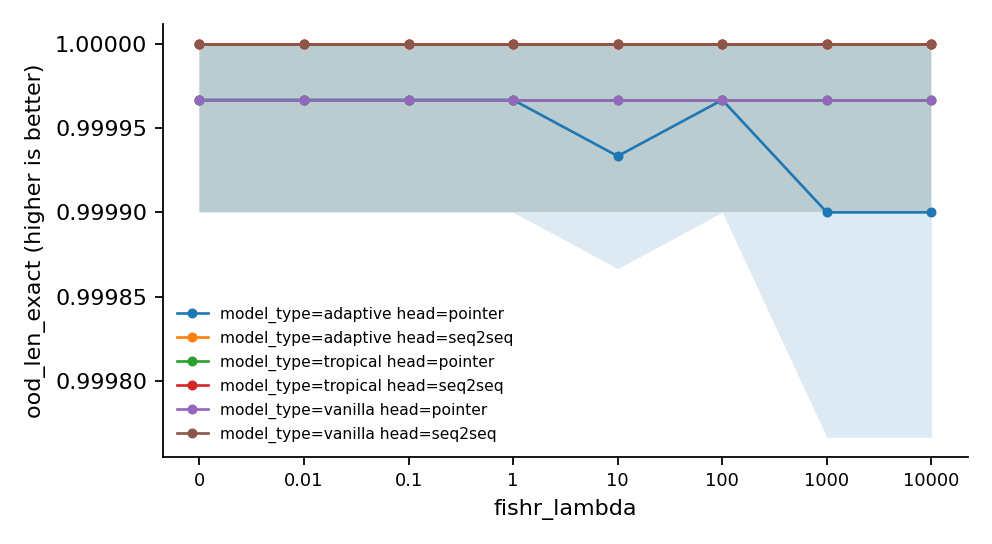
\includegraphics[width=\textwidth]{metric_ood_len_exact.png}
\caption{\texttt{ood\_len\_exact} against \texttt{fishr\_lambda}: the mean over seeds with a 95\% bootstrap CI, one line per combination of the other factors.}
\label{fig:ood_len_exact}
\end{figure}

{\small
\begin{longtable}{lllrlrrr}
\caption{\texttt{ood\_len\_exact} per cell: mean, 95\% bootstrap CI, SD, seeds, diverged runs.}\label{tab:summary-ood_len_exact}\\
\toprule
\texttt{model\_type} & \texttt{head} & \texttt{fishr\_lambda} & mean & 95\% CI & SD & $n$ & div.\\
\midrule
\endhead
adaptive & pointer & 0 & 1 & [1, 1] & $7.45\times10^{-5}$ & 5 & 0\\
adaptive & pointer & 0.01 & 1 & [1, 1] & $7.45\times10^{-5}$ & 5 & 0\\
adaptive & pointer & 0.1 & 1 & [1, 1] & $7.45\times10^{-5}$ & 5 & 0\\
adaptive & pointer & 1 & 1 & [1, 1] & $7.45\times10^{-5}$ & 5 & 0\\
adaptive & pointer & 10 & 0.9999 & [1, 1] & $9.13\times10^{-5}$ & 5 & 0\\
adaptive & pointer & 100 & 1 & [1, 1] & $7.45\times10^{-5}$ & 5 & 0\\
adaptive & pointer & 1000 & 0.9999 & [1, 1] & $1.49\times10^{-4}$ & 5 & 0\\
adaptive & pointer & 1e+04 & 0.9999 & [1, 1] & $1.49\times10^{-4}$ & 5 & 0\\
adaptive & seq2seq & 0 & 1 & [1, 1] & 0 & 5 & 0\\
adaptive & seq2seq & 0.01 & 1 & [1, 1] & 0 & 5 & 0\\
adaptive & seq2seq & 0.1 & 1 & [1, 1] & 0 & 5 & 0\\
adaptive & seq2seq & 1 & 1 & [1, 1] & 0 & 5 & 0\\
adaptive & seq2seq & 10 & 1 & [1, 1] & 0 & 5 & 0\\
adaptive & seq2seq & 100 & 1 & [1, 1] & 0 & 5 & 0\\
adaptive & seq2seq & 1000 & 1 & [1, 1] & 0 & 5 & 0\\
adaptive & seq2seq & 1e+04 & 1 & [1, 1] & 0 & 5 & 0\\
tropical & pointer & 0 & 1 & [1, 1] & $7.45\times10^{-5}$ & 5 & 0\\
tropical & pointer & 0.01 & 1 & [1, 1] & $7.45\times10^{-5}$ & 5 & 0\\
tropical & pointer & 0.1 & 1 & [1, 1] & $7.45\times10^{-5}$ & 5 & 0\\
tropical & pointer & 1 & 1 & [1, 1] & $7.45\times10^{-5}$ & 5 & 0\\
tropical & pointer & 10 & 1 & [1, 1] & $7.45\times10^{-5}$ & 5 & 0\\
tropical & pointer & 100 & 1 & [1, 1] & $7.45\times10^{-5}$ & 5 & 0\\
tropical & pointer & 1000 & 1 & [1, 1] & $7.45\times10^{-5}$ & 5 & 0\\
tropical & pointer & 1e+04 & 1 & [1, 1] & $7.45\times10^{-5}$ & 5 & 0\\
tropical & seq2seq & 0 & 1 & [1, 1] & 0 & 5 & 0\\
tropical & seq2seq & 0.01 & 1 & [1, 1] & 0 & 5 & 0\\
tropical & seq2seq & 0.1 & 1 & [1, 1] & 0 & 5 & 0\\
tropical & seq2seq & 1 & 1 & [1, 1] & 0 & 5 & 0\\
tropical & seq2seq & 10 & 1 & [1, 1] & 0 & 5 & 0\\
tropical & seq2seq & 100 & 1 & [1, 1] & 0 & 5 & 0\\
tropical & seq2seq & 1000 & 1 & [1, 1] & 0 & 5 & 0\\
tropical & seq2seq & 1e+04 & 1 & [1, 1] & 0 & 5 & 0\\
vanilla & pointer & 0 & 1 & [1, 1] & $7.45\times10^{-5}$ & 5 & 0\\
vanilla & pointer & 0.01 & 1 & [1, 1] & $7.45\times10^{-5}$ & 5 & 0\\
vanilla & pointer & 0.1 & 1 & [1, 1] & $7.45\times10^{-5}$ & 5 & 0\\
vanilla & pointer & 1 & 1 & [1, 1] & $7.45\times10^{-5}$ & 5 & 0\\
vanilla & pointer & 10 & 1 & [1, 1] & $7.45\times10^{-5}$ & 5 & 0\\
vanilla & pointer & 100 & 1 & [1, 1] & $7.45\times10^{-5}$ & 5 & 0\\
vanilla & pointer & 1000 & 1 & [1, 1] & $7.45\times10^{-5}$ & 5 & 0\\
vanilla & pointer & 1e+04 & 1 & [1, 1] & $7.45\times10^{-5}$ & 5 & 0\\
vanilla & seq2seq & 0 & 1 & [1, 1] & 0 & 5 & 0\\
vanilla & seq2seq & 0.01 & 1 & [1, 1] & 0 & 5 & 0\\
vanilla & seq2seq & 0.1 & 1 & [1, 1] & 0 & 5 & 0\\
vanilla & seq2seq & 1 & 1 & [1, 1] & 0 & 5 & 0\\
vanilla & seq2seq & 10 & 1 & [1, 1] & 0 & 5 & 0\\
vanilla & seq2seq & 100 & 1 & [1, 1] & 0 & 5 & 0\\
vanilla & seq2seq & 1000 & 1 & [1, 1] & 0 & 5 & 0\\
vanilla & seq2seq & 1e+04 & 1 & [1, 1] & 0 & 5 & 0\\
\bottomrule
\end{longtable}
}

{\small
\begin{longtable}{lllrrrl}
\caption{\texttt{ood\_len\_exact}: each level of \texttt{fishr\_lambda} against its control (0), within each combination of the other factors. rank: Wilcoxon signed-rank by seed, Holm.}\label{tab:control-ood_len_exact}\\
\toprule
\texttt{model\_type} & \texttt{head} & \texttt{fishr\_lambda} & difference & 95\% CI & $p$ & \\
\midrule
\endhead
adaptive & pointer & 0.01 & 0 & [0, 0] & -- & \\
adaptive & pointer & 0.1 & 0 & [0, 0] & -- & \\
adaptive & pointer & 1 & 0 & [0, 0] & -- & \\
adaptive & pointer & 10 & 0 & [$-1.00\times10^{-4}$, 0] & 1.0000 & \\
adaptive & pointer & 100 & 0 & [0, 0] & -- & \\
adaptive & pointer & 1000 & 0 & [$-2.00\times10^{-4}$, 0] & 1.0000 & \\
adaptive & pointer & 1e+04 & 0 & [$-2.00\times10^{-4}$, 0] & 1.0000 & \\
adaptive & seq2seq & 0.01 & 0 & [0, 0] & -- & \\
adaptive & seq2seq & 0.1 & 0 & [0, 0] & -- & \\
adaptive & seq2seq & 1 & 0 & [0, 0] & -- & \\
adaptive & seq2seq & 10 & 0 & [0, 0] & -- & \\
adaptive & seq2seq & 100 & 0 & [0, 0] & -- & \\
adaptive & seq2seq & 1000 & 0 & [0, 0] & -- & \\
adaptive & seq2seq & 1e+04 & 0 & [0, 0] & -- & \\
tropical & pointer & 0.01 & 0 & [0, 0] & -- & \\
tropical & pointer & 0.1 & 0 & [0, 0] & -- & \\
tropical & pointer & 1 & 0 & [0, 0] & -- & \\
tropical & pointer & 10 & 0 & [0, 0] & -- & \\
tropical & pointer & 100 & 0 & [0, 0] & -- & \\
tropical & pointer & 1000 & 0 & [0, 0] & -- & \\
tropical & pointer & 1e+04 & 0 & [0, 0] & -- & \\
tropical & seq2seq & 0.01 & 0 & [0, 0] & -- & \\
tropical & seq2seq & 0.1 & 0 & [0, 0] & -- & \\
tropical & seq2seq & 1 & 0 & [0, 0] & -- & \\
tropical & seq2seq & 10 & 0 & [0, 0] & -- & \\
tropical & seq2seq & 100 & 0 & [0, 0] & -- & \\
tropical & seq2seq & 1000 & 0 & [0, 0] & -- & \\
tropical & seq2seq & 1e+04 & 0 & [0, 0] & -- & \\
vanilla & pointer & 0.01 & 0 & [0, 0] & -- & \\
vanilla & pointer & 0.1 & 0 & [0, 0] & -- & \\
vanilla & pointer & 1 & 0 & [0, 0] & -- & \\
vanilla & pointer & 10 & 0 & [0, 0] & -- & \\
vanilla & pointer & 100 & 0 & [0, 0] & -- & \\
vanilla & pointer & 1000 & 0 & [0, 0] & -- & \\
vanilla & pointer & 1e+04 & 0 & [0, 0] & -- & \\
vanilla & seq2seq & 0.01 & 0 & [0, 0] & -- & \\
vanilla & seq2seq & 0.1 & 0 & [0, 0] & -- & \\
vanilla & seq2seq & 1 & 0 & [0, 0] & -- & \\
vanilla & seq2seq & 10 & 0 & [0, 0] & -- & \\
vanilla & seq2seq & 100 & 0 & [0, 0] & -- & \\
vanilla & seq2seq & 1000 & 0 & [0, 0] & -- & \\
vanilla & seq2seq & 1e+04 & 0 & [0, 0] & -- & \\
\bottomrule
\end{longtable}
}

{\small
\begin{longtable}{llrrrrr}
\caption{\texttt{ood\_len\_exact} against log10 \texttt{fishr\_lambda}: rank: Spearman rho, seed-bootstrap CI, with the Jonckheere--Terpstra ordered-trend $\tau$ and $p$.}\label{tab:trend-ood_len_exact}\\
\toprule
\texttt{model\_type} & \texttt{head} & estimate & 95\% CI & $p$ & JT $\tau$ & JT $p$\\
\midrule
\endhead
adaptive & pointer & -0.1925 & [-0.53, 0] & 0.2679 & -0.118 & 0.2743\\
adaptive & seq2seq & -- & [--, --] & -- & -- & --\\
tropical & pointer & 0 & [0, 0] & 1.0000 & 0 & 1.0000\\
tropical & seq2seq & -- & [--, --] & -- & -- & --\\
vanilla & pointer & 0 & [0, 0] & 1.0000 & 0 & 1.0000\\
vanilla & seq2seq & -- & [--, --] & -- & -- & --\\
\bottomrule
\end{longtable}
}

{\small
\begin{longtable}{lrrrl}
\caption{\texttt{ood\_len\_exact}: paired contrasts by seed, Holm-corrected across the cells. rank: Wilcoxon signed-rank by seed, Holm.}\label{tab:paired-ood_len_exact}\\
\toprule
contrast (within) & difference & 95\% CI & $p$ & \\
\midrule
\endhead
\stackcell{model\_type: tropical - vanilla\\\footnotesize head=pointer fishr\_lambda=0 } & 0 & [--, --] & -- & \\
\stackcell{model\_type: tropical - vanilla\\\footnotesize head=pointer fishr\_lambda=0.01 } & 0 & [--, --] & -- & \\
\stackcell{model\_type: tropical - vanilla\\\footnotesize head=pointer fishr\_lambda=0.1 } & 0 & [--, --] & -- & \\
\stackcell{model\_type: tropical - vanilla\\\footnotesize head=pointer fishr\_lambda=1 } & 0 & [--, --] & -- & \\
\stackcell{model\_type: tropical - vanilla\\\footnotesize head=pointer fishr\_lambda=10 } & 0 & [--, --] & -- & \\
\stackcell{model\_type: tropical - vanilla\\\footnotesize head=pointer fishr\_lambda=100 } & 0 & [--, --] & -- & \\
\stackcell{model\_type: tropical - vanilla\\\footnotesize head=pointer fishr\_lambda=1000 } & 0 & [--, --] & -- & \\
\stackcell{model\_type: tropical - vanilla\\\footnotesize head=pointer fishr\_lambda=1e+04 } & 0 & [--, --] & -- & \\
\stackcell{model\_type: tropical - vanilla\\\footnotesize head=seq2seq fishr\_lambda=0 } & 0 & [--, --] & -- & \\
\stackcell{model\_type: tropical - vanilla\\\footnotesize head=seq2seq fishr\_lambda=0.01 } & 0 & [--, --] & -- & \\
\stackcell{model\_type: tropical - vanilla\\\footnotesize head=seq2seq fishr\_lambda=0.1 } & 0 & [--, --] & -- & \\
\stackcell{model\_type: tropical - vanilla\\\footnotesize head=seq2seq fishr\_lambda=1 } & 0 & [--, --] & -- & \\
\stackcell{model\_type: tropical - vanilla\\\footnotesize head=seq2seq fishr\_lambda=10 } & 0 & [--, --] & -- & \\
\stackcell{model\_type: tropical - vanilla\\\footnotesize head=seq2seq fishr\_lambda=100 } & 0 & [--, --] & -- & \\
\stackcell{model\_type: tropical - vanilla\\\footnotesize head=seq2seq fishr\_lambda=1000 } & 0 & [--, --] & -- & \\
\stackcell{model\_type: tropical - vanilla\\\footnotesize head=seq2seq fishr\_lambda=1e+04 } & 0 & [--, --] & -- & \\
\stackcell{model\_type: adaptive - vanilla\\\footnotesize head=pointer fishr\_lambda=0 } & 0 & [--, --] & -- & \\
\stackcell{model\_type: adaptive - vanilla\\\footnotesize head=pointer fishr\_lambda=0.01 } & 0 & [--, --] & -- & \\
\stackcell{model\_type: adaptive - vanilla\\\footnotesize head=pointer fishr\_lambda=0.1 } & 0 & [--, --] & -- & \\
\stackcell{model\_type: adaptive - vanilla\\\footnotesize head=pointer fishr\_lambda=1 } & 0 & [--, --] & -- & \\
\stackcell{model\_type: adaptive - vanilla\\\footnotesize head=pointer fishr\_lambda=10 } & $-3.333\times10^{-5}$ & [$-1.26\times10^{-4}$, $5.92\times10^{-5}$] & 1.0000 & \\
\stackcell{model\_type: adaptive - vanilla\\\footnotesize head=pointer fishr\_lambda=100 } & 0 & [--, --] & -- & \\
\stackcell{model\_type: adaptive - vanilla\\\footnotesize head=pointer fishr\_lambda=1000 } & $-6.667\times10^{-5}$ & [$-2.52\times10^{-4}$, $1.18\times10^{-4}$] & 1.0000 & \\
\stackcell{model\_type: adaptive - vanilla\\\footnotesize head=pointer fishr\_lambda=1e+04 } & $-6.667\times10^{-5}$ & [$-2.52\times10^{-4}$, $1.18\times10^{-4}$] & 1.0000 & \\
\stackcell{model\_type: adaptive - vanilla\\\footnotesize head=seq2seq fishr\_lambda=0 } & 0 & [--, --] & -- & \\
\stackcell{model\_type: adaptive - vanilla\\\footnotesize head=seq2seq fishr\_lambda=0.01 } & 0 & [--, --] & -- & \\
\stackcell{model\_type: adaptive - vanilla\\\footnotesize head=seq2seq fishr\_lambda=0.1 } & 0 & [--, --] & -- & \\
\stackcell{model\_type: adaptive - vanilla\\\footnotesize head=seq2seq fishr\_lambda=1 } & 0 & [--, --] & -- & \\
\stackcell{model\_type: adaptive - vanilla\\\footnotesize head=seq2seq fishr\_lambda=10 } & 0 & [--, --] & -- & \\
\stackcell{model\_type: adaptive - vanilla\\\footnotesize head=seq2seq fishr\_lambda=100 } & 0 & [--, --] & -- & \\
\stackcell{model\_type: adaptive - vanilla\\\footnotesize head=seq2seq fishr\_lambda=1000 } & 0 & [--, --] & -- & \\
\stackcell{model\_type: adaptive - vanilla\\\footnotesize head=seq2seq fishr\_lambda=1e+04 } & 0 & [--, --] & -- & \\
\stackcell{head: pointer - seq2seq\\\footnotesize model\_type=adaptive fishr\_lambda=0 } & $-3.333\times10^{-5}$ & [$-1.26\times10^{-4}$, $5.92\times10^{-5}$] & 1.0000 & \\
\stackcell{head: pointer - seq2seq\\\footnotesize model\_type=adaptive fishr\_lambda=0.01 } & $-3.333\times10^{-5}$ & [$-1.26\times10^{-4}$, $5.92\times10^{-5}$] & 1.0000 & \\
\stackcell{head: pointer - seq2seq\\\footnotesize model\_type=adaptive fishr\_lambda=0.1 } & $-3.333\times10^{-5}$ & [$-1.26\times10^{-4}$, $5.92\times10^{-5}$] & 1.0000 & \\
\stackcell{head: pointer - seq2seq\\\footnotesize model\_type=adaptive fishr\_lambda=1 } & $-3.333\times10^{-5}$ & [$-1.26\times10^{-4}$, $5.92\times10^{-5}$] & 1.0000 & \\
\stackcell{head: pointer - seq2seq\\\footnotesize model\_type=adaptive fishr\_lambda=10 } & $-6.667\times10^{-5}$ & [$-1.80\times10^{-4}$, $4.67\times10^{-5}$] & 1.0000 & \\
\stackcell{head: pointer - seq2seq\\\footnotesize model\_type=adaptive fishr\_lambda=100 } & $-3.333\times10^{-5}$ & [$-1.26\times10^{-4}$, $5.92\times10^{-5}$] & 1.0000 & \\
\stackcell{head: pointer - seq2seq\\\footnotesize model\_type=adaptive fishr\_lambda=1000 } & $-1.000\times10^{-4}$ & [$-2.85\times10^{-4}$, $8.51\times10^{-5}$] & 1.0000 & \\
\stackcell{head: pointer - seq2seq\\\footnotesize model\_type=adaptive fishr\_lambda=1e+04 } & $-1.000\times10^{-4}$ & [$-2.85\times10^{-4}$, $8.51\times10^{-5}$] & 1.0000 & \\
\stackcell{head: pointer - seq2seq\\\footnotesize model\_type=tropical fishr\_lambda=0 } & $-3.333\times10^{-5}$ & [$-1.26\times10^{-4}$, $5.92\times10^{-5}$] & 1.0000 & \\
\stackcell{head: pointer - seq2seq\\\footnotesize model\_type=tropical fishr\_lambda=0.01 } & $-3.333\times10^{-5}$ & [$-1.26\times10^{-4}$, $5.92\times10^{-5}$] & 1.0000 & \\
\stackcell{head: pointer - seq2seq\\\footnotesize model\_type=tropical fishr\_lambda=0.1 } & $-3.333\times10^{-5}$ & [$-1.26\times10^{-4}$, $5.92\times10^{-5}$] & 1.0000 & \\
\stackcell{head: pointer - seq2seq\\\footnotesize model\_type=tropical fishr\_lambda=1 } & $-3.333\times10^{-5}$ & [$-1.26\times10^{-4}$, $5.92\times10^{-5}$] & 1.0000 & \\
\stackcell{head: pointer - seq2seq\\\footnotesize model\_type=tropical fishr\_lambda=10 } & $-3.333\times10^{-5}$ & [$-1.26\times10^{-4}$, $5.92\times10^{-5}$] & 1.0000 & \\
\stackcell{head: pointer - seq2seq\\\footnotesize model\_type=tropical fishr\_lambda=100 } & $-3.333\times10^{-5}$ & [$-1.26\times10^{-4}$, $5.92\times10^{-5}$] & 1.0000 & \\
\stackcell{head: pointer - seq2seq\\\footnotesize model\_type=tropical fishr\_lambda=1000 } & $-3.333\times10^{-5}$ & [$-1.26\times10^{-4}$, $5.92\times10^{-5}$] & 1.0000 & \\
\stackcell{head: pointer - seq2seq\\\footnotesize model\_type=tropical fishr\_lambda=1e+04 } & $-3.333\times10^{-5}$ & [$-1.26\times10^{-4}$, $5.92\times10^{-5}$] & 1.0000 & \\
\stackcell{head: pointer - seq2seq\\\footnotesize model\_type=vanilla fishr\_lambda=0 } & $-3.333\times10^{-5}$ & [$-1.26\times10^{-4}$, $5.92\times10^{-5}$] & 1.0000 & \\
\stackcell{head: pointer - seq2seq\\\footnotesize model\_type=vanilla fishr\_lambda=0.01 } & $-3.333\times10^{-5}$ & [$-1.26\times10^{-4}$, $5.92\times10^{-5}$] & 1.0000 & \\
\stackcell{head: pointer - seq2seq\\\footnotesize model\_type=vanilla fishr\_lambda=0.1 } & $-3.333\times10^{-5}$ & [$-1.26\times10^{-4}$, $5.92\times10^{-5}$] & 1.0000 & \\
\stackcell{head: pointer - seq2seq\\\footnotesize model\_type=vanilla fishr\_lambda=1 } & $-3.333\times10^{-5}$ & [$-1.26\times10^{-4}$, $5.92\times10^{-5}$] & 1.0000 & \\
\stackcell{head: pointer - seq2seq\\\footnotesize model\_type=vanilla fishr\_lambda=10 } & $-3.333\times10^{-5}$ & [$-1.26\times10^{-4}$, $5.92\times10^{-5}$] & 1.0000 & \\
\stackcell{head: pointer - seq2seq\\\footnotesize model\_type=vanilla fishr\_lambda=100 } & $-3.333\times10^{-5}$ & [$-1.26\times10^{-4}$, $5.92\times10^{-5}$] & 1.0000 & \\
\stackcell{head: pointer - seq2seq\\\footnotesize model\_type=vanilla fishr\_lambda=1000 } & $-3.333\times10^{-5}$ & [$-1.26\times10^{-4}$, $5.92\times10^{-5}$] & 1.0000 & \\
\stackcell{head: pointer - seq2seq\\\footnotesize model\_type=vanilla fishr\_lambda=1e+04 } & $-3.333\times10^{-5}$ & [$-1.26\times10^{-4}$, $5.92\times10^{-5}$] & 1.0000 & \\
\bottomrule
\end{longtable}
}

\subsection{\texttt{ood\_val\_f1}}
\begin{figure}[tbp]
\centering
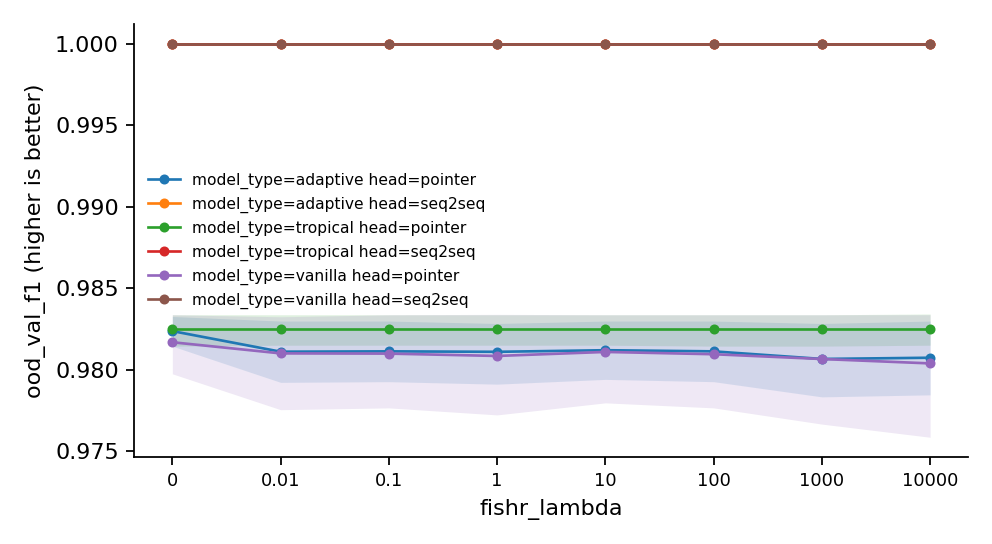
\includegraphics[width=\textwidth]{metric_ood_val_f1.png}
\caption{\texttt{ood\_val\_f1} against \texttt{fishr\_lambda}: the mean over seeds with a 95\% bootstrap CI, one line per combination of the other factors.}
\label{fig:ood_val_f1}
\end{figure}

{\small
\begin{longtable}{lllrlrrr}
\caption{\texttt{ood\_val\_f1} per cell: mean, 95\% bootstrap CI, SD, seeds, diverged runs.}\label{tab:summary-ood_val_f1}\\
\toprule
\texttt{model\_type} & \texttt{head} & \texttt{fishr\_lambda} & mean & 95\% CI & SD & $n$ & div.\\
\midrule
\endhead
adaptive & pointer & 0 & 0.9824 & [0.981, 0.983] & 0.00126 & 5 & 0\\
adaptive & pointer & 0.01 & 0.9811 & [0.979, 0.983] & 0.00238 & 5 & 0\\
adaptive & pointer & 0.1 & 0.9811 & [0.979, 0.983] & 0.00236 & 5 & 0\\
adaptive & pointer & 1 & 0.9811 & [0.979, 0.983] & 0.00239 & 5 & 0\\
adaptive & pointer & 10 & 0.9812 & [0.979, 0.983] & 0.00227 & 5 & 0\\
adaptive & pointer & 100 & 0.9811 & [0.979, 0.983] & 0.00236 & 5 & 0\\
adaptive & pointer & 1000 & 0.9807 & [0.978, 0.983] & 0.00297 & 5 & 0\\
adaptive & pointer & 1e+04 & 0.9807 & [0.978, 0.983] & 0.00298 & 5 & 0\\
adaptive & seq2seq & 0 & 1 & [1, 1] & 0 & 5 & 0\\
adaptive & seq2seq & 0.01 & 1 & [1, 1] & 0 & 5 & 0\\
adaptive & seq2seq & 0.1 & 1 & [1, 1] & 0 & 5 & 0\\
adaptive & seq2seq & 1 & 1 & [1, 1] & 0 & 5 & 0\\
adaptive & seq2seq & 10 & 1 & [1, 1] & 0 & 5 & 0\\
adaptive & seq2seq & 100 & 1 & [1, 1] & 0 & 5 & 0\\
adaptive & seq2seq & 1000 & 1 & [1, 1] & 0 & 5 & 0\\
adaptive & seq2seq & 1e+04 & 1 & [1, 1] & 0 & 5 & 0\\
tropical & pointer & 0 & 0.9825 & [0.981, 0.983] & 0.00124 & 5 & 0\\
tropical & pointer & 0.01 & 0.9825 & [0.981, 0.983] & 0.00124 & 5 & 0\\
tropical & pointer & 0.1 & 0.9825 & [0.981, 0.983] & 0.00124 & 5 & 0\\
tropical & pointer & 1 & 0.9825 & [0.981, 0.983] & 0.00124 & 5 & 0\\
tropical & pointer & 10 & 0.9825 & [0.981, 0.983] & 0.00124 & 5 & 0\\
tropical & pointer & 100 & 0.9825 & [0.981, 0.983] & 0.00124 & 5 & 0\\
tropical & pointer & 1000 & 0.9825 & [0.981, 0.983] & 0.00124 & 5 & 0\\
tropical & pointer & 1e+04 & 0.9825 & [0.981, 0.983] & 0.00124 & 5 & 0\\
tropical & seq2seq & 0 & 1 & [1, 1] & 0 & 5 & 0\\
tropical & seq2seq & 0.01 & 1 & [1, 1] & 0 & 5 & 0\\
tropical & seq2seq & 0.1 & 1 & [1, 1] & 0 & 5 & 0\\
tropical & seq2seq & 1 & 1 & [1, 1] & 0 & 5 & 0\\
tropical & seq2seq & 10 & 1 & [1, 1] & 0 & 5 & 0\\
tropical & seq2seq & 100 & 1 & [1, 1] & 0 & 5 & 0\\
tropical & seq2seq & 1000 & 1 & [1, 1] & 0 & 5 & 0\\
tropical & seq2seq & 1e+04 & 1 & [1, 1] & 0 & 5 & 0\\
vanilla & pointer & 0 & 0.9817 & [0.98, 0.983] & 0.00237 & 5 & 0\\
vanilla & pointer & 0.01 & 0.981 & [0.978, 0.983] & 0.00376 & 5 & 0\\
vanilla & pointer & 0.1 & 0.981 & [0.978, 0.983] & 0.00379 & 5 & 0\\
vanilla & pointer & 1 & 0.9808 & [0.977, 0.983] & 0.0041 & 5 & 0\\
vanilla & pointer & 10 & 0.9811 & [0.978, 0.983] & 0.00357 & 5 & 0\\
vanilla & pointer & 100 & 0.9809 & [0.978, 0.983] & 0.00387 & 5 & 0\\
vanilla & pointer & 1000 & 0.9807 & [0.977, 0.983] & 0.0045 & 5 & 0\\
vanilla & pointer & 1e+04 & 0.9804 & [0.976, 0.983] & 0.00508 & 5 & 0\\
vanilla & seq2seq & 0 & 1 & [1, 1] & 0 & 5 & 0\\
vanilla & seq2seq & 0.01 & 1 & [1, 1] & 0 & 5 & 0\\
vanilla & seq2seq & 0.1 & 1 & [1, 1] & 0 & 5 & 0\\
vanilla & seq2seq & 1 & 1 & [1, 1] & 0 & 5 & 0\\
vanilla & seq2seq & 10 & 1 & [1, 1] & 0 & 5 & 0\\
vanilla & seq2seq & 100 & 1 & [1, 1] & 0 & 5 & 0\\
vanilla & seq2seq & 1000 & 1 & [1, 1] & 0 & 5 & 0\\
vanilla & seq2seq & 1e+04 & 1 & [1, 1] & 0 & 5 & 0\\
\bottomrule
\end{longtable}
}

{\small
\begin{longtable}{lllrrrl}
\caption{\texttt{ood\_val\_f1}: each level of \texttt{fishr\_lambda} against its control (0), within each combination of the other factors. rank: Wilcoxon signed-rank by seed, Holm.}\label{tab:control-ood_val_f1}\\
\toprule
\texttt{model\_type} & \texttt{head} & \texttt{fishr\_lambda} & difference & 95\% CI & $p$ & \\
\midrule
\endhead
adaptive & pointer & 0.01 & 0 & [-0.00259, 0] & 1.0000 & \\
adaptive & pointer & 0.1 & 0 & [-0.00257, 0] & 1.0000 & \\
adaptive & pointer & 1 & 0 & [-0.00265, 0] & 1.0000 & \\
adaptive & pointer & 10 & 0 & [-0.00235, 0] & 1.0000 & \\
adaptive & pointer & 100 & 0 & [-0.0026, 0] & 1.0000 & \\
adaptive & pointer & 1000 & 0 & [-0.00373, 0] & 1.0000 & \\
adaptive & pointer & 1e+04 & 0 & [-0.00379, 0] & 1.0000 & \\
adaptive & seq2seq & 0.01 & 0 & [0, 0] & -- & \\
adaptive & seq2seq & 0.1 & 0 & [0, 0] & -- & \\
adaptive & seq2seq & 1 & 0 & [0, 0] & -- & \\
adaptive & seq2seq & 10 & 0 & [0, 0] & -- & \\
adaptive & seq2seq & 100 & 0 & [0, 0] & -- & \\
adaptive & seq2seq & 1000 & 0 & [0, 0] & -- & \\
adaptive & seq2seq & 1e+04 & 0 & [0, 0] & -- & \\
tropical & pointer & 0.01 & 0 & [0, 0] & -- & \\
tropical & pointer & 0.1 & 0 & [0, 0] & -- & \\
tropical & pointer & 1 & 0 & [0, 0] & -- & \\
tropical & pointer & 10 & 0 & [0, 0] & -- & \\
tropical & pointer & 100 & 0 & [0, 0] & -- & \\
tropical & pointer & 1000 & 0 & [0, 0] & -- & \\
tropical & pointer & 1e+04 & 0 & [0, 0] & -- & \\
tropical & seq2seq & 0.01 & 0 & [0, 0] & -- & \\
tropical & seq2seq & 0.1 & 0 & [0, 0] & -- & \\
tropical & seq2seq & 1 & 0 & [0, 0] & -- & \\
tropical & seq2seq & 10 & 0 & [0, 0] & -- & \\
tropical & seq2seq & 100 & 0 & [0, 0] & -- & \\
tropical & seq2seq & 1000 & 0 & [0, 0] & -- & \\
tropical & seq2seq & 1e+04 & 0 & [0, 0] & -- & \\
vanilla & pointer & 0.01 & 0 & [-0.00205, 0] & 1.0000 & \\
vanilla & pointer & 0.1 & 0 & [-0.00209, 0] & 1.0000 & \\
vanilla & pointer & 1 & 0 & [-0.00252, 0] & 1.0000 & \\
vanilla & pointer & 10 & 0 & [-0.00178, 0] & 1.0000 & \\
vanilla & pointer & 100 & 0 & [-0.00221, 0] & 1.0000 & \\
vanilla & pointer & 1000 & 0 & [-0.00309, 0] & 1.0000 & \\
vanilla & pointer & 1e+04 & 0 & [-0.0039, 0] & 1.0000 & \\
vanilla & seq2seq & 0.01 & 0 & [0, 0] & -- & \\
vanilla & seq2seq & 0.1 & 0 & [0, 0] & -- & \\
vanilla & seq2seq & 1 & 0 & [0, 0] & -- & \\
vanilla & seq2seq & 10 & 0 & [0, 0] & -- & \\
vanilla & seq2seq & 100 & 0 & [0, 0] & -- & \\
vanilla & seq2seq & 1000 & 0 & [0, 0] & -- & \\
vanilla & seq2seq & 1e+04 & 0 & [0, 0] & -- & \\
\bottomrule
\end{longtable}
}

{\small
\begin{longtable}{llrrrrr}
\caption{\texttt{ood\_val\_f1} against log10 \texttt{fishr\_lambda}: rank: Spearman rho, seed-bootstrap CI, with the Jonckheere--Terpstra ordered-trend $\tau$ and $p$.}\label{tab:trend-ood_val_f1}\\
\toprule
\texttt{model\_type} & \texttt{head} & estimate & 95\% CI & $p$ & JT $\tau$ & JT $p$\\
\midrule
\endhead
adaptive & pointer & -0.03078 & [-0.152, 0.0129] & 0.8607 & -0.0248 & 0.8598\\
adaptive & seq2seq & -- & [--, --] & -- & -- & --\\
tropical & pointer & 0 & [0, 0] & 1.0000 & 0 & 1.0000\\
tropical & seq2seq & -- & [--, --] & -- & -- & --\\
vanilla & pointer & -0.02874 & [-0.257, 0] & 0.8698 & -0.0248 & 0.8562\\
vanilla & seq2seq & -- & [--, --] & -- & -- & --\\
\bottomrule
\end{longtable}
}

{\small
\begin{longtable}{lrrrl}
\caption{\texttt{ood\_val\_f1}: paired contrasts by seed, Holm-corrected across the cells. rank: Wilcoxon signed-rank by seed, Holm.}\label{tab:paired-ood_val_f1}\\
\toprule
contrast (within) & difference & 95\% CI & $p$ & \\
\midrule
\endhead
\stackcell{model\_type: tropical - vanilla\\\footnotesize head=pointer fishr\_lambda=0 } & $8.035\times10^{-4}$ & [-0.00143, 0.00303] & 1.0000 & \\
\stackcell{model\_type: tropical - vanilla\\\footnotesize head=pointer fishr\_lambda=0.01 } & 0.001487 & [-0.00264, 0.00562] & 1.0000 & \\
\stackcell{model\_type: tropical - vanilla\\\footnotesize head=pointer fishr\_lambda=0.1 } & 0.001501 & [-0.00267, 0.00567] & 1.0000 & \\
\stackcell{model\_type: tropical - vanilla\\\footnotesize head=pointer fishr\_lambda=1 } & 0.001645 & [-0.00292, 0.00621] & 1.0000 & \\
\stackcell{model\_type: tropical - vanilla\\\footnotesize head=pointer fishr\_lambda=10 } & 0.001398 & [-0.00248, 0.00528] & 1.0000 & \\
\stackcell{model\_type: tropical - vanilla\\\footnotesize head=pointer fishr\_lambda=100 } & 0.001539 & [-0.00273, 0.00581] & 1.0000 & \\
\stackcell{model\_type: tropical - vanilla\\\footnotesize head=pointer fishr\_lambda=1000 } & 0.001833 & [-0.00326, 0.00692] & 1.0000 & \\
\stackcell{model\_type: tropical - vanilla\\\footnotesize head=pointer fishr\_lambda=1e+04 } & 0.002102 & [-0.00373, 0.00794] & 1.0000 & \\
\stackcell{model\_type: tropical - vanilla\\\footnotesize head=seq2seq fishr\_lambda=0 } & 0 & [--, --] & -- & \\
\stackcell{model\_type: tropical - vanilla\\\footnotesize head=seq2seq fishr\_lambda=0.01 } & 0 & [--, --] & -- & \\
\stackcell{model\_type: tropical - vanilla\\\footnotesize head=seq2seq fishr\_lambda=0.1 } & 0 & [--, --] & -- & \\
\stackcell{model\_type: tropical - vanilla\\\footnotesize head=seq2seq fishr\_lambda=1 } & 0 & [--, --] & -- & \\
\stackcell{model\_type: tropical - vanilla\\\footnotesize head=seq2seq fishr\_lambda=10 } & 0 & [--, --] & -- & \\
\stackcell{model\_type: tropical - vanilla\\\footnotesize head=seq2seq fishr\_lambda=100 } & 0 & [--, --] & -- & \\
\stackcell{model\_type: tropical - vanilla\\\footnotesize head=seq2seq fishr\_lambda=1000 } & 0 & [--, --] & -- & \\
\stackcell{model\_type: tropical - vanilla\\\footnotesize head=seq2seq fishr\_lambda=1e+04 } & 0 & [--, --] & -- & \\
\stackcell{model\_type: adaptive - vanilla\\\footnotesize head=pointer fishr\_lambda=0 } & $6.837\times10^{-4}$ & [-0.0016, 0.00297] & 1.0000 & \\
\stackcell{model\_type: adaptive - vanilla\\\footnotesize head=pointer fishr\_lambda=0.01 } & $1.039\times10^{-4}$ & [-0.00349, 0.0037] & 1.0000 & \\
\stackcell{model\_type: adaptive - vanilla\\\footnotesize head=pointer fishr\_lambda=0.1 } & $1.382\times10^{-4}$ & [-0.00355, 0.00383] & 1.0000 & \\
\stackcell{model\_type: adaptive - vanilla\\\footnotesize head=pointer fishr\_lambda=1 } & $2.540\times10^{-4}$ & [-0.00381, 0.00432] & 1.0000 & \\
\stackcell{model\_type: adaptive - vanilla\\\footnotesize head=pointer fishr\_lambda=10 } & $1.056\times10^{-4}$ & [-0.00319, 0.0034] & 1.0000 & \\
\stackcell{model\_type: adaptive - vanilla\\\footnotesize head=pointer fishr\_lambda=100 } & $1.757\times10^{-4}$ & [-0.00366, 0.00401] & 1.0000 & \\
\stackcell{model\_type: adaptive - vanilla\\\footnotesize head=pointer fishr\_lambda=1000 } & $3.736\times10^{-6}$ & [-0.00354, 0.00355] & 1.0000 & \\
\stackcell{model\_type: adaptive - vanilla\\\footnotesize head=pointer fishr\_lambda=1e+04 } & $3.478\times10^{-4}$ & [-0.00337, 0.00406] & 1.0000 & \\
\stackcell{model\_type: adaptive - vanilla\\\footnotesize head=seq2seq fishr\_lambda=0 } & 0 & [--, --] & -- & \\
\stackcell{model\_type: adaptive - vanilla\\\footnotesize head=seq2seq fishr\_lambda=0.01 } & 0 & [--, --] & -- & \\
\stackcell{model\_type: adaptive - vanilla\\\footnotesize head=seq2seq fishr\_lambda=0.1 } & 0 & [--, --] & -- & \\
\stackcell{model\_type: adaptive - vanilla\\\footnotesize head=seq2seq fishr\_lambda=1 } & 0 & [--, --] & -- & \\
\stackcell{model\_type: adaptive - vanilla\\\footnotesize head=seq2seq fishr\_lambda=10 } & 0 & [--, --] & -- & \\
\stackcell{model\_type: adaptive - vanilla\\\footnotesize head=seq2seq fishr\_lambda=100 } & 0 & [--, --] & -- & \\
\stackcell{model\_type: adaptive - vanilla\\\footnotesize head=seq2seq fishr\_lambda=1000 } & 0 & [--, --] & -- & \\
\stackcell{model\_type: adaptive - vanilla\\\footnotesize head=seq2seq fishr\_lambda=1e+04 } & 0 & [--, --] & -- & \\
\stackcell{head: pointer - seq2seq\\\footnotesize model\_type=adaptive fishr\_lambda=0 } & -0.01764 & [-0.0192, -0.0161] & 1.0000 & \\
\stackcell{head: pointer - seq2seq\\\footnotesize model\_type=adaptive fishr\_lambda=0.01 } & -0.0189 & [-0.0219, -0.0159] & 1.0000 & \\
\stackcell{head: pointer - seq2seq\\\footnotesize model\_type=adaptive fishr\_lambda=0.1 } & -0.01888 & [-0.0218, -0.016] & 1.0000 & \\
\stackcell{head: pointer - seq2seq\\\footnotesize model\_type=adaptive fishr\_lambda=1 } & -0.01891 & [-0.0219, -0.0159] & 1.0000 & \\
\stackcell{head: pointer - seq2seq\\\footnotesize model\_type=adaptive fishr\_lambda=10 } & -0.01881 & [-0.0216, -0.016] & 1.0000 & \\
\stackcell{head: pointer - seq2seq\\\footnotesize model\_type=adaptive fishr\_lambda=100 } & -0.01888 & [-0.0218, -0.0159] & 1.0000 & \\
\stackcell{head: pointer - seq2seq\\\footnotesize model\_type=adaptive fishr\_lambda=1000 } & -0.01935 & [-0.023, -0.0157] & 1.0000 & \\
\stackcell{head: pointer - seq2seq\\\footnotesize model\_type=adaptive fishr\_lambda=1e+04 } & -0.01927 & [-0.023, -0.0156] & 1.0000 & \\
\stackcell{head: pointer - seq2seq\\\footnotesize model\_type=tropical fishr\_lambda=0 } & -0.01752 & [-0.0191, -0.016] & 1.0000 & \\
\stackcell{head: pointer - seq2seq\\\footnotesize model\_type=tropical fishr\_lambda=0.01 } & -0.01752 & [-0.0191, -0.016] & 1.0000 & \\
\stackcell{head: pointer - seq2seq\\\footnotesize model\_type=tropical fishr\_lambda=0.1 } & -0.01752 & [-0.0191, -0.016] & 1.0000 & \\
\stackcell{head: pointer - seq2seq\\\footnotesize model\_type=tropical fishr\_lambda=1 } & -0.01752 & [-0.0191, -0.016] & 1.0000 & \\
\stackcell{head: pointer - seq2seq\\\footnotesize model\_type=tropical fishr\_lambda=10 } & -0.01752 & [-0.0191, -0.016] & 1.0000 & \\
\stackcell{head: pointer - seq2seq\\\footnotesize model\_type=tropical fishr\_lambda=100 } & -0.01752 & [-0.0191, -0.016] & 1.0000 & \\
\stackcell{head: pointer - seq2seq\\\footnotesize model\_type=tropical fishr\_lambda=1000 } & -0.01752 & [-0.0191, -0.016] & 1.0000 & \\
\stackcell{head: pointer - seq2seq\\\footnotesize model\_type=tropical fishr\_lambda=1e+04 } & -0.01752 & [-0.0191, -0.016] & 1.0000 & \\
\stackcell{head: pointer - seq2seq\\\footnotesize model\_type=vanilla fishr\_lambda=0 } & -0.01832 & [-0.0213, -0.0154] & 1.0000 & \\
\stackcell{head: pointer - seq2seq\\\footnotesize model\_type=vanilla fishr\_lambda=0.01 } & -0.019 & [-0.0237, -0.0143] & 1.0000 & \\
\stackcell{head: pointer - seq2seq\\\footnotesize model\_type=vanilla fishr\_lambda=0.1 } & -0.01902 & [-0.0237, -0.0143] & 1.0000 & \\
\stackcell{head: pointer - seq2seq\\\footnotesize model\_type=vanilla fishr\_lambda=1 } & -0.01916 & [-0.0242, -0.0141] & 1.0000 & \\
\stackcell{head: pointer - seq2seq\\\footnotesize model\_type=vanilla fishr\_lambda=10 } & -0.01891 & [-0.0234, -0.0145] & 1.0000 & \\
\stackcell{head: pointer - seq2seq\\\footnotesize model\_type=vanilla fishr\_lambda=100 } & -0.01906 & [-0.0239, -0.0142] & 1.0000 & \\
\stackcell{head: pointer - seq2seq\\\footnotesize model\_type=vanilla fishr\_lambda=1000 } & -0.01935 & [-0.0249, -0.0138] & 1.0000 & \\
\stackcell{head: pointer - seq2seq\\\footnotesize model\_type=vanilla fishr\_lambda=1e+04 } & -0.01962 & [-0.0259, -0.0133] & 1.0000 & \\
\bottomrule
\end{longtable}
}

\subsection{\texttt{ood\_val\_exact}}
\begin{figure}[tbp]
\centering
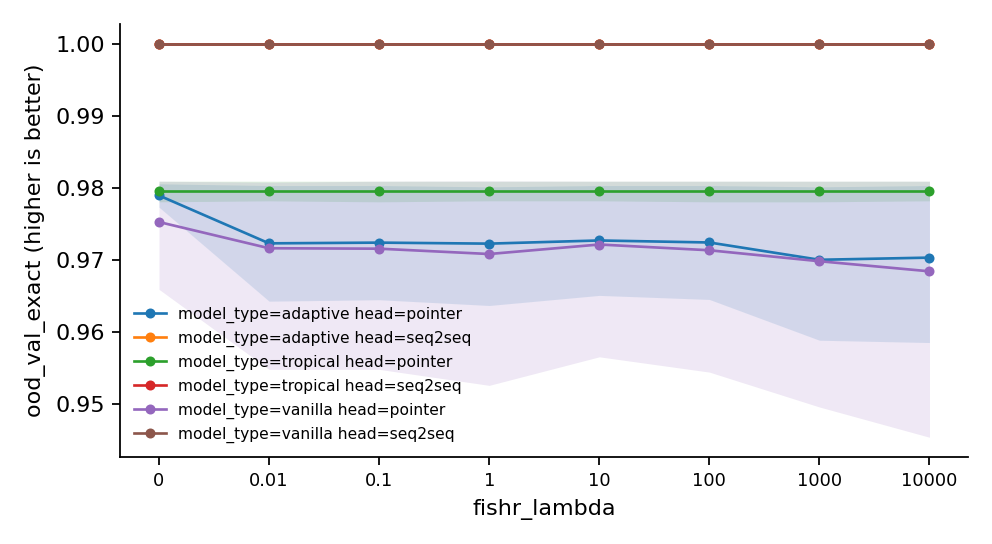
\includegraphics[width=\textwidth]{metric_ood_val_exact.png}
\caption{\texttt{ood\_val\_exact} against \texttt{fishr\_lambda}: the mean over seeds with a 95\% bootstrap CI, one line per combination of the other factors.}
\label{fig:ood_val_exact}
\end{figure}

{\small
\begin{longtable}{lllrlrrr}
\caption{\texttt{ood\_val\_exact} per cell: mean, 95\% bootstrap CI, SD, seeds, diverged runs.}\label{tab:summary-ood_val_exact}\\
\toprule
\texttt{model\_type} & \texttt{head} & \texttt{fishr\_lambda} & mean & 95\% CI & SD & $n$ & div.\\
\midrule
\endhead
adaptive & pointer & 0 & 0.9789 & [0.977, 0.981] & 0.00209 & 5 & 0\\
adaptive & pointer & 0.01 & 0.9723 & [0.964, 0.98] & 0.0104 & 5 & 0\\
adaptive & pointer & 0.1 & 0.9724 & [0.964, 0.98] & 0.0103 & 5 & 0\\
adaptive & pointer & 1 & 0.9723 & [0.964, 0.98] & 0.0105 & 5 & 0\\
adaptive & pointer & 10 & 0.9727 & [0.965, 0.98] & 0.00983 & 5 & 0\\
adaptive & pointer & 100 & 0.9724 & [0.965, 0.98] & 0.0103 & 5 & 0\\
adaptive & pointer & 1000 & 0.97 & [0.959, 0.98] & 0.0138 & 5 & 0\\
adaptive & pointer & 1e+04 & 0.9703 & [0.959, 0.98] & 0.0139 & 5 & 0\\
adaptive & seq2seq & 0 & 1 & [1, 1] & 0 & 5 & 0\\
adaptive & seq2seq & 0.01 & 1 & [1, 1] & 0 & 5 & 0\\
adaptive & seq2seq & 0.1 & 1 & [1, 1] & 0 & 5 & 0\\
adaptive & seq2seq & 1 & 1 & [1, 1] & 0 & 5 & 0\\
adaptive & seq2seq & 10 & 1 & [1, 1] & 0 & 5 & 0\\
adaptive & seq2seq & 100 & 1 & [1, 1] & 0 & 5 & 0\\
adaptive & seq2seq & 1000 & 1 & [1, 1] & 0 & 5 & 0\\
adaptive & seq2seq & 1e+04 & 1 & [1, 1] & 0 & 5 & 0\\
tropical & pointer & 0 & 0.9796 & [0.978, 0.981] & 0.00181 & 5 & 0\\
tropical & pointer & 0.01 & 0.9796 & [0.978, 0.981] & 0.00181 & 5 & 0\\
tropical & pointer & 0.1 & 0.9796 & [0.978, 0.981] & 0.00181 & 5 & 0\\
tropical & pointer & 1 & 0.9796 & [0.978, 0.981] & 0.00181 & 5 & 0\\
tropical & pointer & 10 & 0.9796 & [0.978, 0.981] & 0.00181 & 5 & 0\\
tropical & pointer & 100 & 0.9796 & [0.978, 0.981] & 0.00181 & 5 & 0\\
tropical & pointer & 1000 & 0.9796 & [0.978, 0.981] & 0.00181 & 5 & 0\\
tropical & pointer & 1e+04 & 0.9796 & [0.978, 0.981] & 0.00181 & 5 & 0\\
tropical & seq2seq & 0 & 1 & [1, 1] & 0 & 5 & 0\\
tropical & seq2seq & 0.01 & 1 & [1, 1] & 0 & 5 & 0\\
tropical & seq2seq & 0.1 & 1 & [1, 1] & 0 & 5 & 0\\
tropical & seq2seq & 1 & 1 & [1, 1] & 0 & 5 & 0\\
tropical & seq2seq & 10 & 1 & [1, 1] & 0 & 5 & 0\\
tropical & seq2seq & 100 & 1 & [1, 1] & 0 & 5 & 0\\
tropical & seq2seq & 1000 & 1 & [1, 1] & 0 & 5 & 0\\
tropical & seq2seq & 1e+04 & 1 & [1, 1] & 0 & 5 & 0\\
vanilla & pointer & 0 & 0.9753 & [0.966, 0.981] & 0.0104 & 5 & 0\\
vanilla & pointer & 0.01 & 0.9716 & [0.955, 0.981] & 0.0184 & 5 & 0\\
vanilla & pointer & 0.1 & 0.9716 & [0.955, 0.981] & 0.0186 & 5 & 0\\
vanilla & pointer & 1 & 0.9708 & [0.953, 0.981] & 0.0202 & 5 & 0\\
vanilla & pointer & 10 & 0.9721 & [0.957, 0.981] & 0.0173 & 5 & 0\\
vanilla & pointer & 100 & 0.9713 & [0.954, 0.981] & 0.0191 & 5 & 0\\
vanilla & pointer & 1000 & 0.9698 & [0.95, 0.981] & 0.0224 & 5 & 0\\
vanilla & pointer & 1e+04 & 0.9684 & [0.945, 0.981] & 0.0256 & 5 & 0\\
vanilla & seq2seq & 0 & 1 & [1, 1] & 0 & 5 & 0\\
vanilla & seq2seq & 0.01 & 1 & [1, 1] & 0 & 5 & 0\\
vanilla & seq2seq & 0.1 & 1 & [1, 1] & 0 & 5 & 0\\
vanilla & seq2seq & 1 & 1 & [1, 1] & 0 & 5 & 0\\
vanilla & seq2seq & 10 & 1 & [1, 1] & 0 & 5 & 0\\
vanilla & seq2seq & 100 & 1 & [1, 1] & 0 & 5 & 0\\
vanilla & seq2seq & 1000 & 1 & [1, 1] & 0 & 5 & 0\\
vanilla & seq2seq & 1e+04 & 1 & [1, 1] & 0 & 5 & 0\\
\bottomrule
\end{longtable}
}

{\small
\begin{longtable}{lllrrrl}
\caption{\texttt{ood\_val\_exact}: each level of \texttt{fishr\_lambda} against its control (0), within each combination of the other factors. rank: Wilcoxon signed-rank by seed, Holm.}\label{tab:control-ood_val_exact}\\
\toprule
\texttt{model\_type} & \texttt{head} & \texttt{fishr\_lambda} & difference & 95\% CI & $p$ & \\
\midrule
\endhead
adaptive & pointer & 0.01 & 0 & [-0.0134, 0] & 1.0000 & \\
adaptive & pointer & 0.1 & 0 & [-0.0133, 0] & 1.0000 & \\
adaptive & pointer & 1 & 0 & [-0.0137, 0] & 1.0000 & \\
adaptive & pointer & 10 & 0 & [-0.0126, 0] & 1.0000 & \\
adaptive & pointer & 100 & 0 & [-0.0134, 0] & 1.0000 & \\
adaptive & pointer & 1000 & 0 & [-0.0196, 0] & 1.0000 & \\
adaptive & pointer & 1e+04 & 0 & [-0.0201, 0] & 1.0000 & \\
adaptive & seq2seq & 0.01 & 0 & [0, 0] & -- & \\
adaptive & seq2seq & 0.1 & 0 & [0, 0] & -- & \\
adaptive & seq2seq & 1 & 0 & [0, 0] & -- & \\
adaptive & seq2seq & 10 & 0 & [0, 0] & -- & \\
adaptive & seq2seq & 100 & 0 & [0, 0] & -- & \\
adaptive & seq2seq & 1000 & 0 & [0, 0] & -- & \\
adaptive & seq2seq & 1e+04 & 0 & [0, 0] & -- & \\
tropical & pointer & 0.01 & 0 & [0, 0] & -- & \\
tropical & pointer & 0.1 & 0 & [0, 0] & -- & \\
tropical & pointer & 1 & 0 & [0, 0] & -- & \\
tropical & pointer & 10 & 0 & [0, 0] & -- & \\
tropical & pointer & 100 & 0 & [0, 0] & -- & \\
tropical & pointer & 1000 & 0 & [0, 0] & -- & \\
tropical & pointer & 1e+04 & 0 & [0, 0] & -- & \\
tropical & seq2seq & 0.01 & 0 & [0, 0] & -- & \\
tropical & seq2seq & 0.1 & 0 & [0, 0] & -- & \\
tropical & seq2seq & 1 & 0 & [0, 0] & -- & \\
tropical & seq2seq & 10 & 0 & [0, 0] & -- & \\
tropical & seq2seq & 100 & 0 & [0, 0] & -- & \\
tropical & seq2seq & 1000 & 0 & [0, 0] & -- & \\
tropical & seq2seq & 1e+04 & 0 & [0, 0] & -- & \\
vanilla & pointer & 0.01 & 0 & [-0.0109, 0] & 1.0000 & \\
vanilla & pointer & 0.1 & 0 & [-0.0111, 0] & 1.0000 & \\
vanilla & pointer & 1 & 0 & [-0.0133, 0] & 1.0000 & \\
vanilla & pointer & 10 & 0 & [-0.00936, 0] & 1.0000 & \\
vanilla & pointer & 100 & 0 & [-0.0118, 0] & 1.0000 & \\
vanilla & pointer & 1000 & 0 & [-0.0163, 0] & 1.0000 & \\
vanilla & pointer & 1e+04 & 0 & [-0.0205, 0] & 1.0000 & \\
vanilla & seq2seq & 0.01 & 0 & [0, 0] & -- & \\
vanilla & seq2seq & 0.1 & 0 & [0, 0] & -- & \\
vanilla & seq2seq & 1 & 0 & [0, 0] & -- & \\
vanilla & seq2seq & 10 & 0 & [0, 0] & -- & \\
vanilla & seq2seq & 100 & 0 & [0, 0] & -- & \\
vanilla & seq2seq & 1000 & 0 & [0, 0] & -- & \\
vanilla & seq2seq & 1e+04 & 0 & [0, 0] & -- & \\
\bottomrule
\end{longtable}
}

{\small
\begin{longtable}{llrrrrr}
\caption{\texttt{ood\_val\_exact} against log10 \texttt{fishr\_lambda}: rank: Spearman rho, seed-bootstrap CI, with the Jonckheere--Terpstra ordered-trend $\tau$ and $p$.}\label{tab:trend-ood_val_exact}\\
\toprule
\texttt{model\_type} & \texttt{head} & estimate & 95\% CI & $p$ & JT $\tau$ & JT $p$\\
\midrule
\endhead
adaptive & pointer & -0.03292 & [-0.158, 0.0129] & 0.8511 & -0.0305 & 0.8254\\
adaptive & seq2seq & -- & [--, --] & -- & -- & --\\
tropical & pointer & 0 & [0, 0] & 1.0000 & 0 & 1.0000\\
tropical & seq2seq & -- & [--, --] & -- & -- & --\\
vanilla & pointer & -0.02874 & [-0.257, 0] & 0.8698 & -0.0248 & 0.8562\\
vanilla & seq2seq & -- & [--, --] & -- & -- & --\\
\bottomrule
\end{longtable}
}

{\small
\begin{longtable}{lrrrl}
\caption{\texttt{ood\_val\_exact}: paired contrasts by seed, Holm-corrected across the cells. rank: Wilcoxon signed-rank by seed, Holm.}\label{tab:paired-ood_val_exact}\\
\toprule
contrast (within) & difference & 95\% CI & $p$ & \\
\midrule
\endhead
\stackcell{model\_type: tropical - vanilla\\\footnotesize head=pointer fishr\_lambda=0 } & 0.00432 & [-0.00767, 0.0163] & 1.0000 & \\
\stackcell{model\_type: tropical - vanilla\\\footnotesize head=pointer fishr\_lambda=0.01 } & 0.00796 & [-0.0141, 0.0301] & 1.0000 & \\
\stackcell{model\_type: tropical - vanilla\\\footnotesize head=pointer fishr\_lambda=0.1 } & 0.00802 & [-0.0142, 0.0303] & 1.0000 & \\
\stackcell{model\_type: tropical - vanilla\\\footnotesize head=pointer fishr\_lambda=1 } & 0.00876 & [-0.0156, 0.0331] & 1.0000 & \\
\stackcell{model\_type: tropical - vanilla\\\footnotesize head=pointer fishr\_lambda=10 } & 0.00744 & [-0.0132, 0.0281] & 1.0000 & \\
\stackcell{model\_type: tropical - vanilla\\\footnotesize head=pointer fishr\_lambda=100 } & 0.00824 & [-0.0146, 0.0311] & 1.0000 & \\
\stackcell{model\_type: tropical - vanilla\\\footnotesize head=pointer fishr\_lambda=1000 } & 0.00976 & [-0.0173, 0.0369] & 1.0000 & \\
\stackcell{model\_type: tropical - vanilla\\\footnotesize head=pointer fishr\_lambda=1e+04 } & 0.01116 & [-0.0198, 0.0421] & 1.0000 & \\
\stackcell{model\_type: tropical - vanilla\\\footnotesize head=seq2seq fishr\_lambda=0 } & 0 & [--, --] & -- & \\
\stackcell{model\_type: tropical - vanilla\\\footnotesize head=seq2seq fishr\_lambda=0.01 } & 0 & [--, --] & -- & \\
\stackcell{model\_type: tropical - vanilla\\\footnotesize head=seq2seq fishr\_lambda=0.1 } & 0 & [--, --] & -- & \\
\stackcell{model\_type: tropical - vanilla\\\footnotesize head=seq2seq fishr\_lambda=1 } & 0 & [--, --] & -- & \\
\stackcell{model\_type: tropical - vanilla\\\footnotesize head=seq2seq fishr\_lambda=10 } & 0 & [--, --] & -- & \\
\stackcell{model\_type: tropical - vanilla\\\footnotesize head=seq2seq fishr\_lambda=100 } & 0 & [--, --] & -- & \\
\stackcell{model\_type: tropical - vanilla\\\footnotesize head=seq2seq fishr\_lambda=1000 } & 0 & [--, --] & -- & \\
\stackcell{model\_type: tropical - vanilla\\\footnotesize head=seq2seq fishr\_lambda=1e+04 } & 0 & [--, --] & -- & \\
\stackcell{model\_type: adaptive - vanilla\\\footnotesize head=pointer fishr\_lambda=0 } & 0.00368 & [-0.00857, 0.0159] & 1.0000 & \\
\stackcell{model\_type: adaptive - vanilla\\\footnotesize head=pointer fishr\_lambda=0.01 } & $6.800\times10^{-4}$ & [-0.0181, 0.0194] & 1.0000 & \\
\stackcell{model\_type: adaptive - vanilla\\\footnotesize head=pointer fishr\_lambda=0.1 } & $8.400\times10^{-4}$ & [-0.0184, 0.02] & 1.0000 & \\
\stackcell{model\_type: adaptive - vanilla\\\footnotesize head=pointer fishr\_lambda=1 } & 0.00144 & [-0.0197, 0.0226] & 1.0000 & \\
\stackcell{model\_type: adaptive - vanilla\\\footnotesize head=pointer fishr\_lambda=10 } & $5.600\times10^{-4}$ & [-0.0165, 0.0176] & 1.0000 & \\
\stackcell{model\_type: adaptive - vanilla\\\footnotesize head=pointer fishr\_lambda=100 } & 0.00108 & [-0.0189, 0.0211] & 1.0000 & \\
\stackcell{model\_type: adaptive - vanilla\\\footnotesize head=pointer fishr\_lambda=1000 } & $2.000\times10^{-4}$ & [-0.0183, 0.0187] & 1.0000 & \\
\stackcell{model\_type: adaptive - vanilla\\\footnotesize head=pointer fishr\_lambda=1e+04 } & 0.0019 & [-0.0176, 0.0214] & 1.0000 & \\
\stackcell{model\_type: adaptive - vanilla\\\footnotesize head=seq2seq fishr\_lambda=0 } & 0 & [--, --] & -- & \\
\stackcell{model\_type: adaptive - vanilla\\\footnotesize head=seq2seq fishr\_lambda=0.01 } & 0 & [--, --] & -- & \\
\stackcell{model\_type: adaptive - vanilla\\\footnotesize head=seq2seq fishr\_lambda=0.1 } & 0 & [--, --] & -- & \\
\stackcell{model\_type: adaptive - vanilla\\\footnotesize head=seq2seq fishr\_lambda=1 } & 0 & [--, --] & -- & \\
\stackcell{model\_type: adaptive - vanilla\\\footnotesize head=seq2seq fishr\_lambda=10 } & 0 & [--, --] & -- & \\
\stackcell{model\_type: adaptive - vanilla\\\footnotesize head=seq2seq fishr\_lambda=100 } & 0 & [--, --] & -- & \\
\stackcell{model\_type: adaptive - vanilla\\\footnotesize head=seq2seq fishr\_lambda=1000 } & 0 & [--, --] & -- & \\
\stackcell{model\_type: adaptive - vanilla\\\footnotesize head=seq2seq fishr\_lambda=1e+04 } & 0 & [--, --] & -- & \\
\stackcell{head: pointer - seq2seq\\\footnotesize model\_type=adaptive fishr\_lambda=0 } & -0.02106 & [-0.0237, -0.0185] & 1.0000 & \\
\stackcell{head: pointer - seq2seq\\\footnotesize model\_type=adaptive fishr\_lambda=0.01 } & -0.0277 & [-0.0406, -0.0148] & 1.0000 & \\
\stackcell{head: pointer - seq2seq\\\footnotesize model\_type=adaptive fishr\_lambda=0.1 } & -0.0276 & [-0.0403, -0.0149] & 1.0000 & \\
\stackcell{head: pointer - seq2seq\\\footnotesize model\_type=adaptive fishr\_lambda=1 } & -0.02774 & [-0.0407, -0.0147] & 1.0000 & \\
\stackcell{head: pointer - seq2seq\\\footnotesize model\_type=adaptive fishr\_lambda=10 } & -0.0273 & [-0.0395, -0.0151] & 1.0000 & \\
\stackcell{head: pointer - seq2seq\\\footnotesize model\_type=adaptive fishr\_lambda=100 } & -0.02758 & [-0.0403, -0.0148] & 1.0000 & \\
\stackcell{head: pointer - seq2seq\\\footnotesize model\_type=adaptive fishr\_lambda=1000 } & -0.02998 & [-0.0471, -0.0129] & 1.0000 & \\
\stackcell{head: pointer - seq2seq\\\footnotesize model\_type=adaptive fishr\_lambda=1e+04 } & -0.02968 & [-0.0469, -0.0124] & 1.0000 & \\
\stackcell{head: pointer - seq2seq\\\footnotesize model\_type=tropical fishr\_lambda=0 } & -0.02042 & [-0.0227, -0.0182] & 1.0000 & \\
\stackcell{head: pointer - seq2seq\\\footnotesize model\_type=tropical fishr\_lambda=0.01 } & -0.02042 & [-0.0227, -0.0182] & 1.0000 & \\
\stackcell{head: pointer - seq2seq\\\footnotesize model\_type=tropical fishr\_lambda=0.1 } & -0.02042 & [-0.0227, -0.0182] & 1.0000 & \\
\stackcell{head: pointer - seq2seq\\\footnotesize model\_type=tropical fishr\_lambda=1 } & -0.02042 & [-0.0227, -0.0182] & 1.0000 & \\
\stackcell{head: pointer - seq2seq\\\footnotesize model\_type=tropical fishr\_lambda=10 } & -0.02042 & [-0.0227, -0.0182] & 1.0000 & \\
\stackcell{head: pointer - seq2seq\\\footnotesize model\_type=tropical fishr\_lambda=100 } & -0.02042 & [-0.0227, -0.0182] & 1.0000 & \\
\stackcell{head: pointer - seq2seq\\\footnotesize model\_type=tropical fishr\_lambda=1000 } & -0.02042 & [-0.0227, -0.0182] & 1.0000 & \\
\stackcell{head: pointer - seq2seq\\\footnotesize model\_type=tropical fishr\_lambda=1e+04 } & -0.02042 & [-0.0227, -0.0182] & 1.0000 & \\
\stackcell{head: pointer - seq2seq\\\footnotesize model\_type=vanilla fishr\_lambda=0 } & -0.02474 & [-0.0376, -0.0119] & 1.0000 & \\
\stackcell{head: pointer - seq2seq\\\footnotesize model\_type=vanilla fishr\_lambda=0.01 } & -0.02838 & [-0.0513, -0.0055] & 1.0000 & \\
\stackcell{head: pointer - seq2seq\\\footnotesize model\_type=vanilla fishr\_lambda=0.1 } & -0.02844 & [-0.0515, -0.00539] & 1.0000 & \\
\stackcell{head: pointer - seq2seq\\\footnotesize model\_type=vanilla fishr\_lambda=1 } & -0.02918 & [-0.0543, -0.00409] & 1.0000 & \\
\stackcell{head: pointer - seq2seq\\\footnotesize model\_type=vanilla fishr\_lambda=10 } & -0.02786 & [-0.0493, -0.00642] & 1.0000 & \\
\stackcell{head: pointer - seq2seq\\\footnotesize model\_type=vanilla fishr\_lambda=100 } & -0.02866 & [-0.0523, -0.005] & 1.0000 & \\
\stackcell{head: pointer - seq2seq\\\footnotesize model\_type=vanilla fishr\_lambda=1000 } & -0.03018 & [-0.058, -0.00232] & 1.0000 & \\
\stackcell{head: pointer - seq2seq\\\footnotesize model\_type=vanilla fishr\_lambda=1e+04 } & -0.03158 & [-0.0633, $1.58\times10^{-4}$] & 1.0000 & \\
\bottomrule
\end{longtable}
}

\subsection{\texttt{ood\_noise\_f1}}
\begin{figure}[tbp]
\centering
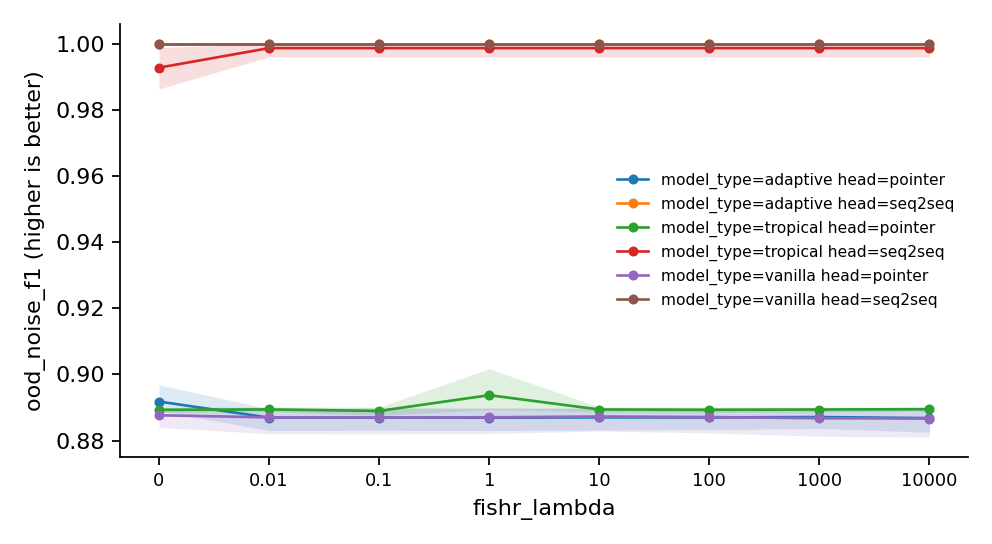
\includegraphics[width=\textwidth]{metric_ood_noise_f1.png}
\caption{\texttt{ood\_noise\_f1} against \texttt{fishr\_lambda}: the mean over seeds with a 95\% bootstrap CI, one line per combination of the other factors.}
\label{fig:ood_noise_f1}
\end{figure}

{\small
\begin{longtable}{lllrlrrr}
\caption{\texttt{ood\_noise\_f1} per cell: mean, 95\% bootstrap CI, SD, seeds, diverged runs.}\label{tab:summary-ood_noise_f1}\\
\toprule
\texttt{model\_type} & \texttt{head} & \texttt{fishr\_lambda} & mean & 95\% CI & SD & $n$ & div.\\
\midrule
\endhead
adaptive & pointer & 0 & 0.8918 & [0.889, 0.897] & 0.00546 & 5 & 0\\
adaptive & pointer & 0.01 & 0.8869 & [0.883, 0.89] & 0.00449 & 5 & 0\\
adaptive & pointer & 0.1 & 0.8869 & [0.883, 0.89] & 0.00445 & 5 & 0\\
adaptive & pointer & 1 & 0.8869 & [0.883, 0.89] & 0.0045 & 5 & 0\\
adaptive & pointer & 10 & 0.887 & [0.883, 0.89] & 0.00439 & 5 & 0\\
adaptive & pointer & 100 & 0.887 & [0.883, 0.89] & 0.00431 & 5 & 0\\
adaptive & pointer & 1000 & 0.8871 & [0.884, 0.89] & 0.00402 & 5 & 0\\
adaptive & pointer & 1e+04 & 0.8868 & [0.883, 0.89] & 0.00492 & 5 & 0\\
adaptive & seq2seq & 0 & 1 & [1, 1] & 0 & 5 & 0\\
adaptive & seq2seq & 0.01 & 1 & [1, 1] & 0 & 5 & 0\\
adaptive & seq2seq & 0.1 & 1 & [1, 1] & 0 & 5 & 0\\
adaptive & seq2seq & 1 & 1 & [1, 1] & 0 & 5 & 0\\
adaptive & seq2seq & 10 & 1 & [1, 1] & 0 & 5 & 0\\
adaptive & seq2seq & 100 & 1 & [1, 1] & 0 & 5 & 0\\
adaptive & seq2seq & 1000 & 1 & [1, 1] & 0 & 5 & 0\\
adaptive & seq2seq & 1e+04 & 1 & [1, 1] & 0 & 5 & 0\\
tropical & pointer & 0 & 0.8893 & [0.888, 0.89] & 0.00102 & 5 & 0\\
tropical & pointer & 0.01 & 0.8894 & [0.889, 0.89] & $9.29\times10^{-4}$ & 5 & 0\\
tropical & pointer & 0.1 & 0.889 & [0.888, 0.89] & 0.00166 & 5 & 0\\
tropical & pointer & 1 & 0.8937 & [0.889, 0.902] & 0.0089 & 5 & 0\\
tropical & pointer & 10 & 0.8894 & [0.889, 0.89] & $9.71\times10^{-4}$ & 5 & 0\\
tropical & pointer & 100 & 0.8893 & [0.888, 0.89] & 0.00109 & 5 & 0\\
tropical & pointer & 1000 & 0.8894 & [0.889, 0.89] & 0.00101 & 5 & 0\\
tropical & pointer & 1e+04 & 0.8895 & [0.889, 0.89] & $8.27\times10^{-4}$ & 5 & 0\\
tropical & seq2seq & 0 & 0.9928 & [0.986, 0.999] & 0.0081 & 5 & 0\\
tropical & seq2seq & 0.01 & 0.9987 & [0.996, 1] & 0.003 & 5 & 0\\
tropical & seq2seq & 0.1 & 0.9987 & [0.996, 1] & 0.003 & 5 & 0\\
tropical & seq2seq & 1 & 0.9987 & [0.996, 1] & 0.003 & 5 & 0\\
tropical & seq2seq & 10 & 0.9987 & [0.996, 1] & 0.003 & 5 & 0\\
tropical & seq2seq & 100 & 0.9987 & [0.996, 1] & 0.003 & 5 & 0\\
tropical & seq2seq & 1000 & 0.9987 & [0.996, 1] & 0.003 & 5 & 0\\
tropical & seq2seq & 1e+04 & 0.9987 & [0.996, 1] & 0.003 & 5 & 0\\
vanilla & pointer & 0 & 0.8877 & [0.884, 0.89] & 0.00403 & 5 & 0\\
vanilla & pointer & 0.01 & 0.887 & [0.882, 0.89] & 0.00546 & 5 & 0\\
vanilla & pointer & 0.1 & 0.887 & [0.882, 0.89] & 0.00549 & 5 & 0\\
vanilla & pointer & 1 & 0.887 & [0.882, 0.89] & 0.00539 & 5 & 0\\
vanilla & pointer & 10 & 0.8873 & [0.883, 0.89] & 0.00486 & 5 & 0\\
vanilla & pointer & 100 & 0.8871 & [0.882, 0.89] & 0.00521 & 5 & 0\\
vanilla & pointer & 1000 & 0.8868 & [0.881, 0.89] & 0.00602 & 5 & 0\\
vanilla & pointer & 1e+04 & 0.8867 & [0.881, 0.89] & 0.00624 & 5 & 0\\
vanilla & seq2seq & 0 & 1 & [1, 1] & 0 & 5 & 0\\
vanilla & seq2seq & 0.01 & 1 & [1, 1] & 0 & 5 & 0\\
vanilla & seq2seq & 0.1 & 1 & [1, 1] & 0 & 5 & 0\\
vanilla & seq2seq & 1 & 1 & [1, 1] & 0 & 5 & 0\\
vanilla & seq2seq & 10 & 1 & [1, 1] & 0 & 5 & 0\\
vanilla & seq2seq & 100 & 1 & [1, 1] & 0 & 5 & 0\\
vanilla & seq2seq & 1000 & 1 & [1, 1] & 0 & 5 & 0\\
vanilla & seq2seq & 1e+04 & 1 & [1, 1] & 0 & 5 & 0\\
\bottomrule
\end{longtable}
}

{\small
\begin{longtable}{lllrrrl}
\caption{\texttt{ood\_noise\_f1}: each level of \texttt{fishr\_lambda} against its control (0), within each combination of the other factors. rank: Wilcoxon signed-rank by seed, Holm.}\label{tab:control-ood_noise_f1}\\
\toprule
\texttt{model\_type} & \texttt{head} & \texttt{fishr\_lambda} & difference & 95\% CI & $p$ & \\
\midrule
\endhead
adaptive & pointer & 0.01 & 0 & [-0.0107, 0] & 1.0000 & \\
adaptive & pointer & 0.1 & 0 & [-0.0107, 0] & 1.0000 & \\
adaptive & pointer & 1 & 0 & [-0.0107, 0] & 1.0000 & \\
adaptive & pointer & 10 & 0 & [-0.0106, 0] & 1.0000 & \\
adaptive & pointer & 100 & 0 & [-0.0107, 0] & 1.0000 & \\
adaptive & pointer & 1000 & 0 & [-0.0106, 0] & 1.0000 & \\
adaptive & pointer & 1e+04 & 0 & [-0.0107, 0] & 1.0000 & \\
adaptive & seq2seq & 0.01 & 0 & [0, 0] & -- & \\
adaptive & seq2seq & 0.1 & 0 & [0, 0] & -- & \\
adaptive & seq2seq & 1 & 0 & [0, 0] & -- & \\
adaptive & seq2seq & 10 & 0 & [0, 0] & -- & \\
adaptive & seq2seq & 100 & 0 & [0, 0] & -- & \\
adaptive & seq2seq & 1000 & 0 & [0, 0] & -- & \\
adaptive & seq2seq & 1e+04 & 0 & [0, 0] & -- & \\
tropical & pointer & 0.01 & 0 & [$-1.83\times10^{-4}$, $5.76\times10^{-4}$] & 1.0000 & \\
tropical & pointer & 0.1 & 0 & [-0.00132, $4.36\times10^{-4}$] & 1.0000 & \\
tropical & pointer & 1 & $6.813\times10^{-5}$ & [$4.55\times10^{-6}$, 0.0129] & 1.0000 & \\
tropical & pointer & 10 & 0 & [$-2.59\times10^{-4}$, $5.78\times10^{-4}$] & 1.0000 & \\
tropical & pointer & 100 & 0 & [$-4.45\times10^{-4}$, $5.27\times10^{-4}$] & 1.0000 & \\
tropical & pointer & 1000 & 0 & [$-3.32\times10^{-4}$, $6.21\times10^{-4}$] & 1.0000 & \\
tropical & pointer & 1e+04 & $6.784\times10^{-5}$ & [$-4.53\times10^{-5}$, $6.14\times10^{-4}$] & 1.0000 & \\
tropical & seq2seq & 0.01 & 0.005907 & [0.00118, 0.0106] & 1.0000 & \\
tropical & seq2seq & 0.1 & 0.005907 & [0.00118, 0.0106] & 1.0000 & \\
tropical & seq2seq & 1 & 0.005907 & [0.00118, 0.0106] & 1.0000 & \\
tropical & seq2seq & 10 & 0.005907 & [0.00118, 0.0106] & 1.0000 & \\
tropical & seq2seq & 100 & 0.005907 & [0.00118, 0.0106] & 1.0000 & \\
tropical & seq2seq & 1000 & 0.005907 & [0.00118, 0.0106] & 1.0000 & \\
tropical & seq2seq & 1e+04 & 0.005907 & [0.00118, 0.0106] & 1.0000 & \\
vanilla & pointer & 0.01 & 0 & [-0.00193, 0] & 1.0000 & \\
vanilla & pointer & 0.1 & 0 & [-0.00197, 0] & 1.0000 & \\
vanilla & pointer & 1 & 0 & [-0.00185, 0] & 1.0000 & \\
vanilla & pointer & 10 & 0 & [-0.00113, 0] & 1.0000 & \\
vanilla & pointer & 100 & 0 & [-0.0016, 0] & 1.0000 & \\
vanilla & pointer & 1000 & 0 & [-0.0027, 0] & 1.0000 & \\
vanilla & pointer & 1e+04 & 0 & [-0.00299, 0] & 1.0000 & \\
vanilla & seq2seq & 0.01 & 0 & [0, 0] & -- & \\
vanilla & seq2seq & 0.1 & 0 & [0, 0] & -- & \\
vanilla & seq2seq & 1 & 0 & [0, 0] & -- & \\
vanilla & seq2seq & 10 & 0 & [0, 0] & -- & \\
vanilla & seq2seq & 100 & 0 & [0, 0] & -- & \\
vanilla & seq2seq & 1000 & 0 & [0, 0] & -- & \\
vanilla & seq2seq & 1e+04 & 0 & [0, 0] & -- & \\
\bottomrule
\end{longtable}
}

{\small
\begin{longtable}{llrrrrr}
\caption{\texttt{ood\_noise\_f1} against log10 \texttt{fishr\_lambda}: rank: Spearman rho, seed-bootstrap CI, with the Jonckheere--Terpstra ordered-trend $\tau$ and $p$.}\label{tab:trend-ood_noise_f1}\\
\toprule
\texttt{model\_type} & \texttt{head} & estimate & 95\% CI & $p$ & JT $\tau$ & JT $p$\\
\midrule
\endhead
adaptive & pointer & 0.004294 & [-0.0129, 0.0514] & 0.9805 & 0.00381 & 0.9844\\
adaptive & seq2seq & -- & [--, --] & -- & -- & --\\
tropical & pointer & -0.01279 & [-0.155, 0.161] & 0.9419 & -0.0114 & 0.9394\\
tropical & seq2seq & 0 & [0, 0] & 1.0000 & 0 & 1.0000\\
vanilla & pointer & -0.01437 & [-0.129, 0] & 0.9347 & -0.00952 & 0.9508\\
vanilla & seq2seq & -- & [--, --] & -- & -- & --\\
\bottomrule
\end{longtable}
}

{\small
\begin{longtable}{lrrrl}
\caption{\texttt{ood\_noise\_f1}: paired contrasts by seed, Holm-corrected across the cells. rank: Wilcoxon signed-rank by seed, Holm.}\label{tab:paired-ood_noise_f1}\\
\toprule
contrast (within) & difference & 95\% CI & $p$ & \\
\midrule
\endhead
\stackcell{model\_type: tropical - vanilla\\\footnotesize head=pointer fishr\_lambda=0 } & 0.001636 & [-0.00391, 0.00718] & 1.0000 & \\
\stackcell{model\_type: tropical - vanilla\\\footnotesize head=pointer fishr\_lambda=0.01 } & 0.002408 & [-0.00482, 0.00963] & 1.0000 & \\
\stackcell{model\_type: tropical - vanilla\\\footnotesize head=pointer fishr\_lambda=0.1 } & 0.001955 & [-0.00573, 0.00964] & 1.0000 & \\
\stackcell{model\_type: tropical - vanilla\\\footnotesize head=pointer fishr\_lambda=1 } & 0.006687 & [-0.00527, 0.0186] & 1.0000 & \\
\stackcell{model\_type: tropical - vanilla\\\footnotesize head=pointer fishr\_lambda=10 } & 0.002117 & [-0.00438, 0.00862] & 1.0000 & \\
\stackcell{model\_type: tropical - vanilla\\\footnotesize head=pointer fishr\_lambda=100 } & 0.002187 & [-0.00482, 0.00919] & 1.0000 & \\
\stackcell{model\_type: tropical - vanilla\\\footnotesize head=pointer fishr\_lambda=1000 } & 0.002635 & [-0.00532, 0.0106] & 1.0000 & \\
\stackcell{model\_type: tropical - vanilla\\\footnotesize head=pointer fishr\_lambda=1e+04 } & 0.002839 & [-0.00531, 0.011] & 1.0000 & \\
\stackcell{model\_type: tropical - vanilla\\\footnotesize head=seq2seq fishr\_lambda=0 } & -0.00725 & [-0.0173, 0.00281] & 1.0000 & \\
\stackcell{model\_type: tropical - vanilla\\\footnotesize head=seq2seq fishr\_lambda=0.01 } & -0.00134 & [-0.00506, 0.00238] & 1.0000 & \\
\stackcell{model\_type: tropical - vanilla\\\footnotesize head=seq2seq fishr\_lambda=0.1 } & -0.00134 & [-0.00506, 0.00238] & 1.0000 & \\
\stackcell{model\_type: tropical - vanilla\\\footnotesize head=seq2seq fishr\_lambda=1 } & -0.00134 & [-0.00506, 0.00238] & 1.0000 & \\
\stackcell{model\_type: tropical - vanilla\\\footnotesize head=seq2seq fishr\_lambda=10 } & -0.00134 & [-0.00506, 0.00238] & 1.0000 & \\
\stackcell{model\_type: tropical - vanilla\\\footnotesize head=seq2seq fishr\_lambda=100 } & -0.00134 & [-0.00506, 0.00238] & 1.0000 & \\
\stackcell{model\_type: tropical - vanilla\\\footnotesize head=seq2seq fishr\_lambda=1000 } & -0.00134 & [-0.00506, 0.00238] & 1.0000 & \\
\stackcell{model\_type: tropical - vanilla\\\footnotesize head=seq2seq fishr\_lambda=1e+04 } & -0.00134 & [-0.00506, 0.00238] & 1.0000 & \\
\stackcell{model\_type: adaptive - vanilla\\\footnotesize head=pointer fishr\_lambda=0 } & 0.004142 & [-0.0031, 0.0114] & 1.0000 & \\
\stackcell{model\_type: adaptive - vanilla\\\footnotesize head=pointer fishr\_lambda=0.01 } & $-7.061\times10^{-5}$ & [-0.00192, 0.00178] & 1.0000 & \\
\stackcell{model\_type: adaptive - vanilla\\\footnotesize head=pointer fishr\_lambda=0.1 } & $-5.307\times10^{-5}$ & [-0.002, 0.0019] & 1.0000 & \\
\stackcell{model\_type: adaptive - vanilla\\\footnotesize head=pointer fishr\_lambda=1 } & $-1.174\times10^{-4}$ & [-0.00194, 0.00171] & 1.0000 & \\
\stackcell{model\_type: adaptive - vanilla\\\footnotesize head=pointer fishr\_lambda=10 } & $-2.617\times10^{-4}$ & [-0.00163, 0.00111] & 1.0000 & \\
\stackcell{model\_type: adaptive - vanilla\\\footnotesize head=pointer fishr\_lambda=100 } & $-1.239\times10^{-4}$ & [-0.002, 0.00175] & 1.0000 & \\
\stackcell{model\_type: adaptive - vanilla\\\footnotesize head=pointer fishr\_lambda=1000 } & $3.598\times10^{-4}$ & [-0.00272, 0.00344] & 1.0000 & \\
\stackcell{model\_type: adaptive - vanilla\\\footnotesize head=pointer fishr\_lambda=1e+04 } & $1.405\times10^{-4}$ & [-0.00193, 0.00221] & 1.0000 & \\
\stackcell{model\_type: adaptive - vanilla\\\footnotesize head=seq2seq fishr\_lambda=0 } & 0 & [--, --] & -- & \\
\stackcell{model\_type: adaptive - vanilla\\\footnotesize head=seq2seq fishr\_lambda=0.01 } & 0 & [--, --] & -- & \\
\stackcell{model\_type: adaptive - vanilla\\\footnotesize head=seq2seq fishr\_lambda=0.1 } & 0 & [--, --] & -- & \\
\stackcell{model\_type: adaptive - vanilla\\\footnotesize head=seq2seq fishr\_lambda=1 } & 0 & [--, --] & -- & \\
\stackcell{model\_type: adaptive - vanilla\\\footnotesize head=seq2seq fishr\_lambda=10 } & 0 & [--, --] & -- & \\
\stackcell{model\_type: adaptive - vanilla\\\footnotesize head=seq2seq fishr\_lambda=100 } & 0 & [--, --] & -- & \\
\stackcell{model\_type: adaptive - vanilla\\\footnotesize head=seq2seq fishr\_lambda=1000 } & 0 & [--, --] & -- & \\
\stackcell{model\_type: adaptive - vanilla\\\footnotesize head=seq2seq fishr\_lambda=1e+04 } & 0 & [--, --] & -- & \\
\stackcell{head: pointer - seq2seq\\\footnotesize model\_type=adaptive fishr\_lambda=0 } & -0.1082 & [-0.115, -0.101] & 1.0000 & \\
\stackcell{head: pointer - seq2seq\\\footnotesize model\_type=adaptive fishr\_lambda=0.01 } & -0.1131 & [-0.119, -0.107] & 1.0000 & \\
\stackcell{head: pointer - seq2seq\\\footnotesize model\_type=adaptive fishr\_lambda=0.1 } & -0.1131 & [-0.119, -0.108] & 1.0000 & \\
\stackcell{head: pointer - seq2seq\\\footnotesize model\_type=adaptive fishr\_lambda=1 } & -0.1131 & [-0.119, -0.107] & 1.0000 & \\
\stackcell{head: pointer - seq2seq\\\footnotesize model\_type=adaptive fishr\_lambda=10 } & -0.113 & [-0.118, -0.108] & 1.0000 & \\
\stackcell{head: pointer - seq2seq\\\footnotesize model\_type=adaptive fishr\_lambda=100 } & -0.113 & [-0.118, -0.108] & 1.0000 & \\
\stackcell{head: pointer - seq2seq\\\footnotesize model\_type=adaptive fishr\_lambda=1000 } & -0.1129 & [-0.118, -0.108] & 1.0000 & \\
\stackcell{head: pointer - seq2seq\\\footnotesize model\_type=adaptive fishr\_lambda=1e+04 } & -0.1132 & [-0.119, -0.107] & 1.0000 & \\
\stackcell{head: pointer - seq2seq\\\footnotesize model\_type=tropical fishr\_lambda=0 } & -0.1035 & [-0.113, -0.0936] & 1.0000 & \\
\stackcell{head: pointer - seq2seq\\\footnotesize model\_type=tropical fishr\_lambda=0.01 } & -0.1092 & [-0.112, -0.106] & 1.0000 & \\
\stackcell{head: pointer - seq2seq\\\footnotesize model\_type=tropical fishr\_lambda=0.1 } & -0.1097 & [-0.112, -0.108] & 1.0000 & \\
\stackcell{head: pointer - seq2seq\\\footnotesize model\_type=tropical fishr\_lambda=1 } & -0.1049 & [-0.12, -0.0902] & 1.0000 & \\
\stackcell{head: pointer - seq2seq\\\footnotesize model\_type=tropical fishr\_lambda=10 } & -0.1093 & [-0.112, -0.106] & 1.0000 & \\
\stackcell{head: pointer - seq2seq\\\footnotesize model\_type=tropical fishr\_lambda=100 } & -0.1093 & [-0.112, -0.107] & 1.0000 & \\
\stackcell{head: pointer - seq2seq\\\footnotesize model\_type=tropical fishr\_lambda=1000 } & -0.1093 & [-0.112, -0.106] & 1.0000 & \\
\stackcell{head: pointer - seq2seq\\\footnotesize model\_type=tropical fishr\_lambda=1e+04 } & -0.1092 & [-0.112, -0.106] & 1.0000 & \\
\stackcell{head: pointer - seq2seq\\\footnotesize model\_type=vanilla fishr\_lambda=0 } & -0.1123 & [-0.117, -0.107] & 1.0000 & \\
\stackcell{head: pointer - seq2seq\\\footnotesize model\_type=vanilla fishr\_lambda=0.01 } & -0.113 & [-0.12, -0.106] & 1.0000 & \\
\stackcell{head: pointer - seq2seq\\\footnotesize model\_type=vanilla fishr\_lambda=0.1 } & -0.113 & [-0.12, -0.106] & 1.0000 & \\
\stackcell{head: pointer - seq2seq\\\footnotesize model\_type=vanilla fishr\_lambda=1 } & -0.113 & [-0.12, -0.106] & 1.0000 & \\
\stackcell{head: pointer - seq2seq\\\footnotesize model\_type=vanilla fishr\_lambda=10 } & -0.1127 & [-0.119, -0.107] & 1.0000 & \\
\stackcell{head: pointer - seq2seq\\\footnotesize model\_type=vanilla fishr\_lambda=100 } & -0.1129 & [-0.119, -0.106] & 1.0000 & \\
\stackcell{head: pointer - seq2seq\\\footnotesize model\_type=vanilla fishr\_lambda=1000 } & -0.1132 & [-0.121, -0.106] & 1.0000 & \\
\stackcell{head: pointer - seq2seq\\\footnotesize model\_type=vanilla fishr\_lambda=1e+04 } & -0.1133 & [-0.121, -0.106] & 1.0000 & \\
\bottomrule
\end{longtable}
}

\subsection{\texttt{ood\_noise\_exact}}
\begin{figure}[tbp]
\centering
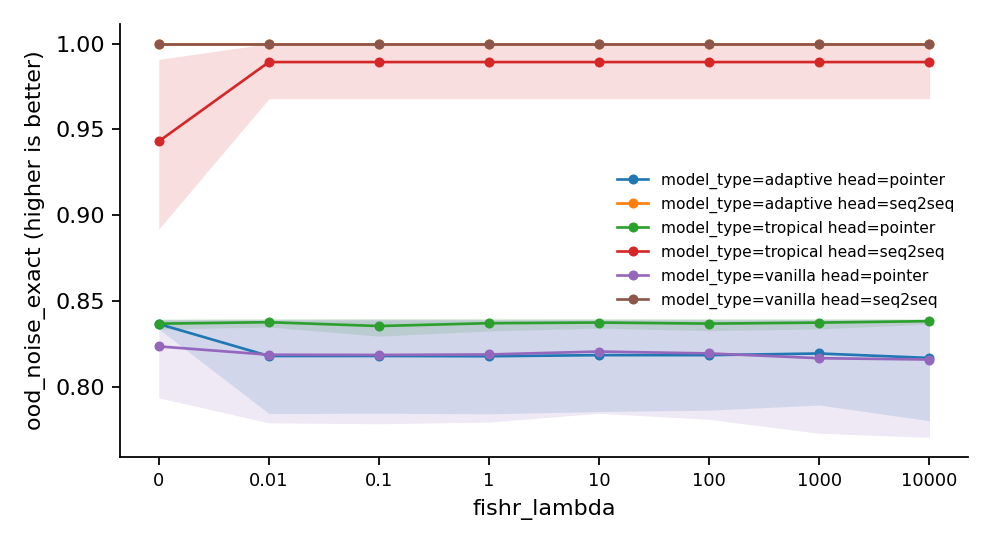
\includegraphics[width=\textwidth]{metric_ood_noise_exact.png}
\caption{\texttt{ood\_noise\_exact} against \texttt{fishr\_lambda}: the mean over seeds with a 95\% bootstrap CI, one line per combination of the other factors.}
\label{fig:ood_noise_exact}
\end{figure}

{\small
\begin{longtable}{lllrlrrr}
\caption{\texttt{ood\_noise\_exact} per cell: mean, 95\% bootstrap CI, SD, seeds, diverged runs.}\label{tab:summary-ood_noise_exact}\\
\toprule
\texttt{model\_type} & \texttt{head} & \texttt{fishr\_lambda} & mean & 95\% CI & SD & $n$ & div.\\
\midrule
\endhead
adaptive & pointer & 0 & 0.8365 & [0.834, 0.839] & 0.00344 & 5 & 0\\
adaptive & pointer & 0.01 & 0.8178 & [0.784, 0.839] & 0.0367 & 5 & 0\\
adaptive & pointer & 0.1 & 0.8178 & [0.784, 0.839] & 0.0365 & 5 & 0\\
adaptive & pointer & 1 & 0.8177 & [0.784, 0.839] & 0.0367 & 5 & 0\\
adaptive & pointer & 10 & 0.8183 & [0.785, 0.839] & 0.036 & 5 & 0\\
adaptive & pointer & 100 & 0.8183 & [0.786, 0.839] & 0.0351 & 5 & 0\\
adaptive & pointer & 1000 & 0.8193 & [0.789, 0.839] & 0.0329 & 5 & 0\\
adaptive & pointer & 1e+04 & 0.8167 & [0.78, 0.839] & 0.0401 & 5 & 0\\
adaptive & seq2seq & 0 & 1 & [1, 1] & 0 & 5 & 0\\
adaptive & seq2seq & 0.01 & 1 & [1, 1] & 0 & 5 & 0\\
adaptive & seq2seq & 0.1 & 1 & [1, 1] & 0 & 5 & 0\\
adaptive & seq2seq & 1 & 1 & [1, 1] & 0 & 5 & 0\\
adaptive & seq2seq & 10 & 1 & [1, 1] & 0 & 5 & 0\\
adaptive & seq2seq & 100 & 1 & [1, 1] & 0 & 5 & 0\\
adaptive & seq2seq & 1000 & 1 & [1, 1] & 0 & 5 & 0\\
adaptive & seq2seq & 1e+04 & 1 & [1, 1] & 0 & 5 & 0\\
tropical & pointer & 0 & 0.8367 & [0.833, 0.839] & 0.00375 & 5 & 0\\
tropical & pointer & 0.01 & 0.8375 & [0.835, 0.84] & 0.00328 & 5 & 0\\
tropical & pointer & 0.1 & 0.8353 & [0.829, 0.84] & 0.00654 & 5 & 0\\
tropical & pointer & 1 & 0.8369 & [0.832, 0.84] & 0.00503 & 5 & 0\\
tropical & pointer & 10 & 0.8373 & [0.834, 0.84] & 0.00369 & 5 & 0\\
tropical & pointer & 100 & 0.8367 & [0.833, 0.84] & 0.0047 & 5 & 0\\
tropical & pointer & 1000 & 0.8373 & [0.834, 0.84] & 0.00418 & 5 & 0\\
tropical & pointer & 1e+04 & 0.8381 & [0.836, 0.84] & 0.00211 & 5 & 0\\
tropical & seq2seq & 0 & 0.943 & [0.892, 0.991] & 0.064 & 5 & 0\\
tropical & seq2seq & 0.01 & 0.9893 & [0.968, 1] & 0.024 & 5 & 0\\
tropical & seq2seq & 0.1 & 0.9893 & [0.968, 1] & 0.024 & 5 & 0\\
tropical & seq2seq & 1 & 0.9893 & [0.968, 1] & 0.024 & 5 & 0\\
tropical & seq2seq & 10 & 0.9893 & [0.968, 1] & 0.024 & 5 & 0\\
tropical & seq2seq & 100 & 0.9893 & [0.968, 1] & 0.024 & 5 & 0\\
tropical & seq2seq & 1000 & 0.9893 & [0.968, 1] & 0.024 & 5 & 0\\
tropical & seq2seq & 1e+04 & 0.9893 & [0.968, 1] & 0.024 & 5 & 0\\
vanilla & pointer & 0 & 0.8234 & [0.793, 0.839] & 0.0336 & 5 & 0\\
vanilla & pointer & 0.01 & 0.8186 & [0.779, 0.839] & 0.0444 & 5 & 0\\
vanilla & pointer & 0.1 & 0.8184 & [0.778, 0.839] & 0.0447 & 5 & 0\\
vanilla & pointer & 1 & 0.8187 & [0.779, 0.839] & 0.0441 & 5 & 0\\
vanilla & pointer & 10 & 0.8204 & [0.784, 0.839] & 0.0403 & 5 & 0\\
vanilla & pointer & 100 & 0.8193 & [0.781, 0.839] & 0.0427 & 5 & 0\\
vanilla & pointer & 1000 & 0.8165 & [0.773, 0.839] & 0.049 & 5 & 0\\
vanilla & pointer & 1e+04 & 0.8158 & [0.77, 0.839] & 0.0507 & 5 & 0\\
vanilla & seq2seq & 0 & 1 & [1, 1] & 0 & 5 & 0\\
vanilla & seq2seq & 0.01 & 1 & [1, 1] & 0 & 5 & 0\\
vanilla & seq2seq & 0.1 & 1 & [1, 1] & 0 & 5 & 0\\
vanilla & seq2seq & 1 & 1 & [1, 1] & 0 & 5 & 0\\
vanilla & seq2seq & 10 & 1 & [1, 1] & 0 & 5 & 0\\
vanilla & seq2seq & 100 & 1 & [1, 1] & 0 & 5 & 0\\
vanilla & seq2seq & 1000 & 1 & [1, 1] & 0 & 5 & 0\\
vanilla & seq2seq & 1e+04 & 1 & [1, 1] & 0 & 5 & 0\\
\bottomrule
\end{longtable}
}

{\small
\begin{longtable}{lllrrrl}
\caption{\texttt{ood\_noise\_exact}: each level of \texttt{fishr\_lambda} against its control (0), within each combination of the other factors. rank: Wilcoxon signed-rank by seed, Holm.}\label{tab:control-ood_noise_exact}\\
\toprule
\texttt{model\_type} & \texttt{head} & \texttt{fishr\_lambda} & difference & 95\% CI & $p$ & \\
\midrule
\endhead
adaptive & pointer & 0.01 & 0 & [-0.0464, 0] & 1.0000 & \\
adaptive & pointer & 0.1 & 0 & [-0.0461, 0] & 1.0000 & \\
adaptive & pointer & 1 & 0 & [-0.0464, 0] & 1.0000 & \\
adaptive & pointer & 10 & 0 & [-0.0454, 0] & 1.0000 & \\
adaptive & pointer & 100 & 0 & [-0.0442, 0] & 1.0000 & \\
adaptive & pointer & 1000 & 0 & [-0.0411, 0] & 1.0000 & \\
adaptive & pointer & 1e+04 & 0 & [-0.051, 0] & 1.0000 & \\
adaptive & seq2seq & 0.01 & 0 & [0, 0] & -- & \\
adaptive & seq2seq & 0.1 & 0 & [0, 0] & -- & \\
adaptive & seq2seq & 1 & 0 & [0, 0] & -- & \\
adaptive & seq2seq & 10 & 0 & [0, 0] & -- & \\
adaptive & seq2seq & 100 & 0 & [0, 0] & -- & \\
adaptive & seq2seq & 1000 & 0 & [0, 0] & -- & \\
adaptive & seq2seq & 1e+04 & 0 & [0, 0] & -- & \\
tropical & pointer & 0.01 & 0 & [-0.00144, 0.00404] & 1.0000 & \\
tropical & pointer & 0.1 & 0 & [-0.00588, 0.00315] & 1.0000 & \\
tropical & pointer & 1 & $-1.000\times10^{-4}$ & [-0.0038, 0.0044] & 1.0000 & \\
tropical & pointer & 10 & 0 & [-0.00204, 0.00406] & 1.0000 & \\
tropical & pointer & 100 & 0 & [-0.0034, 0.00369] & 1.0000 & \\
tropical & pointer & 1000 & 0 & [-0.0027, 0.00444] & 1.0000 & \\
tropical & pointer & 1e+04 & $6.000\times10^{-4}$ & [$-4.00\times10^{-4}$, 0.00438] & 1.0000 & \\
tropical & seq2seq & 0.01 & 0.0458 & [0.00916, 0.0833] & 1.0000 & \\
tropical & seq2seq & 0.1 & 0.0458 & [0.00916, 0.0833] & 1.0000 & \\
tropical & seq2seq & 1 & 0.0458 & [0.00916, 0.0833] & 1.0000 & \\
tropical & seq2seq & 10 & 0.0458 & [0.00916, 0.0833] & 1.0000 & \\
tropical & seq2seq & 100 & 0.0458 & [0.00916, 0.0833] & 1.0000 & \\
tropical & seq2seq & 1000 & 0.0458 & [0.00916, 0.0833] & 1.0000 & \\
tropical & seq2seq & 1e+04 & 0.0458 & [0.00916, 0.0833] & 1.0000 & \\
vanilla & pointer & 0.01 & 0 & [-0.0146, 0] & 1.0000 & \\
vanilla & pointer & 0.1 & 0 & [-0.0149, 0] & 1.0000 & \\
vanilla & pointer & 1 & 0 & [-0.0141, 0] & 1.0000 & \\
vanilla & pointer & 10 & 0 & [-0.009, 0] & 1.0000 & \\
vanilla & pointer & 100 & 0 & [-0.0123, 0] & 1.0000 & \\
vanilla & pointer & 1000 & 0 & [-0.0207, 0] & 1.0000 & \\
vanilla & pointer & 1e+04 & 0 & [-0.023, 0] & 1.0000 & \\
vanilla & seq2seq & 0.01 & 0 & [0, 0] & -- & \\
vanilla & seq2seq & 0.1 & 0 & [0, 0] & -- & \\
vanilla & seq2seq & 1 & 0 & [0, 0] & -- & \\
vanilla & seq2seq & 10 & 0 & [0, 0] & -- & \\
vanilla & seq2seq & 100 & 0 & [0, 0] & -- & \\
vanilla & seq2seq & 1000 & 0 & [0, 0] & -- & \\
vanilla & seq2seq & 1e+04 & 0 & [0, 0] & -- & \\
\bottomrule
\end{longtable}
}

{\small
\begin{longtable}{llrrrrr}
\caption{\texttt{ood\_noise\_exact} against log10 \texttt{fishr\_lambda}: rank: Spearman rho, seed-bootstrap CI, with the Jonckheere--Terpstra ordered-trend $\tau$ and $p$.}\label{tab:trend-ood_noise_exact}\\
\toprule
\texttt{model\_type} & \texttt{head} & estimate & 95\% CI & $p$ & JT $\tau$ & JT $p$\\
\midrule
\endhead
adaptive & pointer & 0.004294 & [-0.0129, 0.0514] & 0.9805 & 0.00381 & 0.9844\\
adaptive & seq2seq & -- & [--, --] & -- & -- & --\\
tropical & pointer & 0.03553 & [-0.139, 0.195] & 0.8394 & 0.0267 & 0.8438\\
tropical & seq2seq & 0 & [0, 0] & 1.0000 & 0 & 1.0000\\
vanilla & pointer & -0.01437 & [-0.129, 0] & 0.9347 & -0.00952 & 0.9454\\
vanilla & seq2seq & -- & [--, --] & -- & -- & --\\
\bottomrule
\end{longtable}
}

{\small
\begin{longtable}{lrrrl}
\caption{\texttt{ood\_noise\_exact}: paired contrasts by seed, Holm-corrected across the cells. rank: Wilcoxon signed-rank by seed, Holm.}\label{tab:paired-ood_noise_exact}\\
\toprule
contrast (within) & difference & 95\% CI & $p$ & \\
\midrule
\endhead
\stackcell{model\_type: tropical - vanilla\\\footnotesize head=pointer fishr\_lambda=0 } & 0.01326 & [-0.0311, 0.0577] & 1.0000 & \\
\stackcell{model\_type: tropical - vanilla\\\footnotesize head=pointer fishr\_lambda=0.01 } & 0.01896 & [-0.0382, 0.0762] & 1.0000 & \\
\stackcell{model\_type: tropical - vanilla\\\footnotesize head=pointer fishr\_lambda=0.1 } & 0.01686 & [-0.0425, 0.0762] & 1.0000 & \\
\stackcell{model\_type: tropical - vanilla\\\footnotesize head=pointer fishr\_lambda=1 } & 0.01822 & [-0.039, 0.0754] & 1.0000 & \\
\stackcell{model\_type: tropical - vanilla\\\footnotesize head=pointer fishr\_lambda=10 } & 0.01692 & [-0.0353, 0.0691] & 1.0000 & \\
\stackcell{model\_type: tropical - vanilla\\\footnotesize head=pointer fishr\_lambda=100 } & 0.01738 & [-0.0384, 0.0731] & 1.0000 & \\
\stackcell{model\_type: tropical - vanilla\\\footnotesize head=pointer fishr\_lambda=1000 } & 0.02078 & [-0.0423, 0.0838] & 1.0000 & \\
\stackcell{model\_type: tropical - vanilla\\\footnotesize head=pointer fishr\_lambda=1e+04 } & 0.02238 & [-0.0421, 0.0869] & 1.0000 & \\
\stackcell{model\_type: tropical - vanilla\\\footnotesize head=seq2seq fishr\_lambda=0 } & -0.05696 & [-0.136, 0.0225] & 1.0000 & \\
\stackcell{model\_type: tropical - vanilla\\\footnotesize head=seq2seq fishr\_lambda=0.01 } & -0.01072 & [-0.0405, 0.019] & 1.0000 & \\
\stackcell{model\_type: tropical - vanilla\\\footnotesize head=seq2seq fishr\_lambda=0.1 } & -0.01072 & [-0.0405, 0.019] & 1.0000 & \\
\stackcell{model\_type: tropical - vanilla\\\footnotesize head=seq2seq fishr\_lambda=1 } & -0.01072 & [-0.0405, 0.019] & 1.0000 & \\
\stackcell{model\_type: tropical - vanilla\\\footnotesize head=seq2seq fishr\_lambda=10 } & -0.01072 & [-0.0405, 0.019] & 1.0000 & \\
\stackcell{model\_type: tropical - vanilla\\\footnotesize head=seq2seq fishr\_lambda=100 } & -0.01072 & [-0.0405, 0.019] & 1.0000 & \\
\stackcell{model\_type: tropical - vanilla\\\footnotesize head=seq2seq fishr\_lambda=1000 } & -0.01072 & [-0.0405, 0.019] & 1.0000 & \\
\stackcell{model\_type: tropical - vanilla\\\footnotesize head=seq2seq fishr\_lambda=1e+04 } & -0.01072 & [-0.0405, 0.019] & 1.0000 & \\
\stackcell{model\_type: adaptive - vanilla\\\footnotesize head=pointer fishr\_lambda=0 } & 0.01306 & [-0.025, 0.0511] & 1.0000 & \\
\stackcell{model\_type: adaptive - vanilla\\\footnotesize head=pointer fishr\_lambda=0.01 } & $-7.400\times10^{-4}$ & [-0.0154, 0.0139] & 1.0000 & \\
\stackcell{model\_type: adaptive - vanilla\\\footnotesize head=pointer fishr\_lambda=0.1 } & $-6.200\times10^{-4}$ & [-0.016, 0.0147] & 1.0000 & \\
\stackcell{model\_type: adaptive - vanilla\\\footnotesize head=pointer fishr\_lambda=1 } & -0.00104 & [-0.0156, 0.0136] & 1.0000 & \\
\stackcell{model\_type: adaptive - vanilla\\\footnotesize head=pointer fishr\_lambda=10 } & -0.0021 & [-0.0136, 0.0094] & 1.0000 & \\
\stackcell{model\_type: adaptive - vanilla\\\footnotesize head=pointer fishr\_lambda=100 } & -0.001 & [-0.0161, 0.0141] & 1.0000 & \\
\stackcell{model\_type: adaptive - vanilla\\\footnotesize head=pointer fishr\_lambda=1000 } & 0.00276 & [-0.0213, 0.0268] & 1.0000 & \\
\stackcell{model\_type: adaptive - vanilla\\\footnotesize head=pointer fishr\_lambda=1e+04 } & $9.000\times10^{-4}$ & [-0.0157, 0.0175] & 1.0000 & \\
\stackcell{model\_type: adaptive - vanilla\\\footnotesize head=seq2seq fishr\_lambda=0 } & 0 & [--, --] & -- & \\
\stackcell{model\_type: adaptive - vanilla\\\footnotesize head=seq2seq fishr\_lambda=0.01 } & 0 & [--, --] & -- & \\
\stackcell{model\_type: adaptive - vanilla\\\footnotesize head=seq2seq fishr\_lambda=0.1 } & 0 & [--, --] & -- & \\
\stackcell{model\_type: adaptive - vanilla\\\footnotesize head=seq2seq fishr\_lambda=1 } & 0 & [--, --] & -- & \\
\stackcell{model\_type: adaptive - vanilla\\\footnotesize head=seq2seq fishr\_lambda=10 } & 0 & [--, --] & -- & \\
\stackcell{model\_type: adaptive - vanilla\\\footnotesize head=seq2seq fishr\_lambda=100 } & 0 & [--, --] & -- & \\
\stackcell{model\_type: adaptive - vanilla\\\footnotesize head=seq2seq fishr\_lambda=1000 } & 0 & [--, --] & -- & \\
\stackcell{model\_type: adaptive - vanilla\\\footnotesize head=seq2seq fishr\_lambda=1e+04 } & 0 & [--, --] & -- & \\
\stackcell{head: pointer - seq2seq\\\footnotesize model\_type=adaptive fishr\_lambda=0 } & -0.1635 & [-0.168, -0.159] & 1.0000 & \\
\stackcell{head: pointer - seq2seq\\\footnotesize model\_type=adaptive fishr\_lambda=0.01 } & -0.1822 & [-0.228, -0.137] & 1.0000 & \\
\stackcell{head: pointer - seq2seq\\\footnotesize model\_type=adaptive fishr\_lambda=0.1 } & -0.1822 & [-0.227, -0.137] & 1.0000 & \\
\stackcell{head: pointer - seq2seq\\\footnotesize model\_type=adaptive fishr\_lambda=1 } & -0.1823 & [-0.228, -0.137] & 1.0000 & \\
\stackcell{head: pointer - seq2seq\\\footnotesize model\_type=adaptive fishr\_lambda=10 } & -0.1817 & [-0.226, -0.137] & 1.0000 & \\
\stackcell{head: pointer - seq2seq\\\footnotesize model\_type=adaptive fishr\_lambda=100 } & -0.1817 & [-0.225, -0.138] & 1.0000 & \\
\stackcell{head: pointer - seq2seq\\\footnotesize model\_type=adaptive fishr\_lambda=1000 } & -0.1807 & [-0.222, -0.14] & 1.0000 & \\
\stackcell{head: pointer - seq2seq\\\footnotesize model\_type=adaptive fishr\_lambda=1e+04 } & -0.1833 & [-0.233, -0.134] & 1.0000 & \\
\stackcell{head: pointer - seq2seq\\\footnotesize model\_type=tropical fishr\_lambda=0 } & -0.1064 & [-0.184, -0.0284] & 1.0000 & \\
\stackcell{head: pointer - seq2seq\\\footnotesize model\_type=tropical fishr\_lambda=0.01 } & -0.1518 & [-0.178, -0.126] & 1.0000 & \\
\stackcell{head: pointer - seq2seq\\\footnotesize model\_type=tropical fishr\_lambda=0.1 } & -0.154 & [-0.177, -0.131] & 1.0000 & \\
\stackcell{head: pointer - seq2seq\\\footnotesize model\_type=tropical fishr\_lambda=1 } & -0.1523 & [-0.176, -0.129] & 1.0000 & \\
\stackcell{head: pointer - seq2seq\\\footnotesize model\_type=tropical fishr\_lambda=10 } & -0.1519 & [-0.177, -0.126] & 1.0000 & \\
\stackcell{head: pointer - seq2seq\\\footnotesize model\_type=tropical fishr\_lambda=100 } & -0.1526 & [-0.177, -0.128] & 1.0000 & \\
\stackcell{head: pointer - seq2seq\\\footnotesize model\_type=tropical fishr\_lambda=1000 } & -0.152 & [-0.177, -0.127] & 1.0000 & \\
\stackcell{head: pointer - seq2seq\\\footnotesize model\_type=tropical fishr\_lambda=1e+04 } & -0.1511 & [-0.179, -0.123] & 1.0000 & \\
\stackcell{head: pointer - seq2seq\\\footnotesize model\_type=vanilla fishr\_lambda=0 } & -0.1766 & [-0.218, -0.135] & 1.0000 & \\
\stackcell{head: pointer - seq2seq\\\footnotesize model\_type=vanilla fishr\_lambda=0.01 } & -0.1814 & [-0.237, -0.126] & 1.0000 & \\
\stackcell{head: pointer - seq2seq\\\footnotesize model\_type=vanilla fishr\_lambda=0.1 } & -0.1816 & [-0.237, -0.126] & 1.0000 & \\
\stackcell{head: pointer - seq2seq\\\footnotesize model\_type=vanilla fishr\_lambda=1 } & -0.1813 & [-0.236, -0.127] & 1.0000 & \\
\stackcell{head: pointer - seq2seq\\\footnotesize model\_type=vanilla fishr\_lambda=10 } & -0.1796 & [-0.23, -0.13] & 1.0000 & \\
\stackcell{head: pointer - seq2seq\\\footnotesize model\_type=vanilla fishr\_lambda=100 } & -0.1807 & [-0.234, -0.128] & 1.0000 & \\
\stackcell{head: pointer - seq2seq\\\footnotesize model\_type=vanilla fishr\_lambda=1000 } & -0.1835 & [-0.244, -0.123] & 1.0000 & \\
\stackcell{head: pointer - seq2seq\\\footnotesize model\_type=vanilla fishr\_lambda=1e+04 } & -0.1842 & [-0.247, -0.121] & 1.0000 & \\
\bottomrule
\end{longtable}
}

\subsection{\texttt{id\_f1}}
\begin{figure}[tbp]
\centering
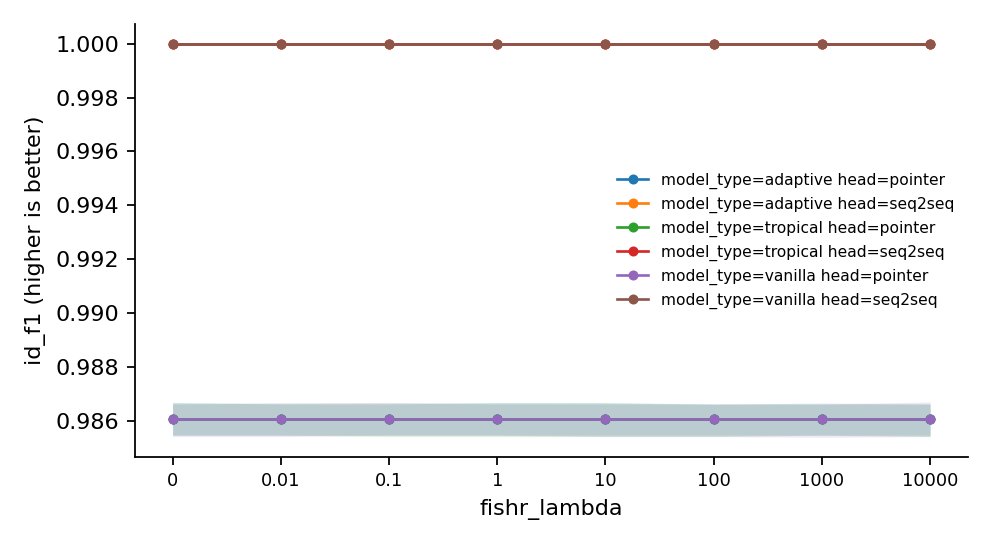
\includegraphics[width=\textwidth]{metric_id_f1.png}
\caption{\texttt{id\_f1} against \texttt{fishr\_lambda}: the mean over seeds with a 95\% bootstrap CI, one line per combination of the other factors.}
\label{fig:id_f1}
\end{figure}

{\small
\begin{longtable}{lllrlrrr}
\caption{\texttt{id\_f1} per cell: mean, 95\% bootstrap CI, SD, seeds, diverged runs.}\label{tab:summary-id_f1}\\
\toprule
\texttt{model\_type} & \texttt{head} & \texttt{fishr\_lambda} & mean & 95\% CI & SD & $n$ & div.\\
\midrule
\endhead
adaptive & pointer & 0 & 0.9861 & [0.985, 0.987] & $7.86\times10^{-4}$ & 5 & 0\\
adaptive & pointer & 0.01 & 0.9861 & [0.985, 0.987] & $7.86\times10^{-4}$ & 5 & 0\\
adaptive & pointer & 0.1 & 0.9861 & [0.985, 0.987] & $7.86\times10^{-4}$ & 5 & 0\\
adaptive & pointer & 1 & 0.9861 & [0.985, 0.987] & $7.86\times10^{-4}$ & 5 & 0\\
adaptive & pointer & 10 & 0.9861 & [0.985, 0.987] & $7.86\times10^{-4}$ & 5 & 0\\
adaptive & pointer & 100 & 0.9861 & [0.985, 0.987] & $7.86\times10^{-4}$ & 5 & 0\\
adaptive & pointer & 1000 & 0.9861 & [0.985, 0.987] & $7.86\times10^{-4}$ & 5 & 0\\
adaptive & pointer & 1e+04 & 0.9861 & [0.985, 0.987] & $7.86\times10^{-4}$ & 5 & 0\\
adaptive & seq2seq & 0 & 1 & [1, 1] & 0 & 5 & 0\\
adaptive & seq2seq & 0.01 & 1 & [1, 1] & 0 & 5 & 0\\
adaptive & seq2seq & 0.1 & 1 & [1, 1] & 0 & 5 & 0\\
adaptive & seq2seq & 1 & 1 & [1, 1] & 0 & 5 & 0\\
adaptive & seq2seq & 10 & 1 & [1, 1] & 0 & 5 & 0\\
adaptive & seq2seq & 100 & 1 & [1, 1] & 0 & 5 & 0\\
adaptive & seq2seq & 1000 & 1 & [1, 1] & 0 & 5 & 0\\
adaptive & seq2seq & 1e+04 & 1 & [1, 1] & 0 & 5 & 0\\
tropical & pointer & 0 & 0.9861 & [0.985, 0.987] & $7.86\times10^{-4}$ & 5 & 0\\
tropical & pointer & 0.01 & 0.9861 & [0.985, 0.987] & $7.86\times10^{-4}$ & 5 & 0\\
tropical & pointer & 0.1 & 0.9861 & [0.985, 0.987] & $7.86\times10^{-4}$ & 5 & 0\\
tropical & pointer & 1 & 0.9861 & [0.985, 0.987] & $7.86\times10^{-4}$ & 5 & 0\\
tropical & pointer & 10 & 0.9861 & [0.985, 0.987] & $7.86\times10^{-4}$ & 5 & 0\\
tropical & pointer & 100 & 0.9861 & [0.985, 0.987] & $7.86\times10^{-4}$ & 5 & 0\\
tropical & pointer & 1000 & 0.9861 & [0.985, 0.987] & $7.86\times10^{-4}$ & 5 & 0\\
tropical & pointer & 1e+04 & 0.9861 & [0.985, 0.987] & $7.86\times10^{-4}$ & 5 & 0\\
tropical & seq2seq & 0 & 1 & [1, 1] & 0 & 5 & 0\\
tropical & seq2seq & 0.01 & 1 & [1, 1] & 0 & 5 & 0\\
tropical & seq2seq & 0.1 & 1 & [1, 1] & 0 & 5 & 0\\
tropical & seq2seq & 1 & 1 & [1, 1] & 0 & 5 & 0\\
tropical & seq2seq & 10 & 1 & [1, 1] & 0 & 5 & 0\\
tropical & seq2seq & 100 & 1 & [1, 1] & 0 & 5 & 0\\
tropical & seq2seq & 1000 & 1 & [1, 1] & 0 & 5 & 0\\
tropical & seq2seq & 1e+04 & 1 & [1, 1] & 0 & 5 & 0\\
vanilla & pointer & 0 & 0.9861 & [0.985, 0.987] & $7.86\times10^{-4}$ & 5 & 0\\
vanilla & pointer & 0.01 & 0.9861 & [0.985, 0.987] & $7.86\times10^{-4}$ & 5 & 0\\
vanilla & pointer & 0.1 & 0.9861 & [0.985, 0.987] & $7.86\times10^{-4}$ & 5 & 0\\
vanilla & pointer & 1 & 0.9861 & [0.985, 0.987] & $7.86\times10^{-4}$ & 5 & 0\\
vanilla & pointer & 10 & 0.9861 & [0.985, 0.987] & $7.86\times10^{-4}$ & 5 & 0\\
vanilla & pointer & 100 & 0.9861 & [0.985, 0.987] & $7.86\times10^{-4}$ & 5 & 0\\
vanilla & pointer & 1000 & 0.9861 & [0.985, 0.987] & $7.86\times10^{-4}$ & 5 & 0\\
vanilla & pointer & 1e+04 & 0.9861 & [0.985, 0.987] & $7.86\times10^{-4}$ & 5 & 0\\
vanilla & seq2seq & 0 & 1 & [1, 1] & 0 & 5 & 0\\
vanilla & seq2seq & 0.01 & 1 & [1, 1] & 0 & 5 & 0\\
vanilla & seq2seq & 0.1 & 1 & [1, 1] & 0 & 5 & 0\\
vanilla & seq2seq & 1 & 1 & [1, 1] & 0 & 5 & 0\\
vanilla & seq2seq & 10 & 1 & [1, 1] & 0 & 5 & 0\\
vanilla & seq2seq & 100 & 1 & [1, 1] & 0 & 5 & 0\\
vanilla & seq2seq & 1000 & 1 & [1, 1] & 0 & 5 & 0\\
vanilla & seq2seq & 1e+04 & 1 & [1, 1] & 0 & 5 & 0\\
\bottomrule
\end{longtable}
}

{\small
\begin{longtable}{lllrrrl}
\caption{\texttt{id\_f1}: each level of \texttt{fishr\_lambda} against its control (0), within each combination of the other factors. rank: Wilcoxon signed-rank by seed, Holm.}\label{tab:control-id_f1}\\
\toprule
\texttt{model\_type} & \texttt{head} & \texttt{fishr\_lambda} & difference & 95\% CI & $p$ & \\
\midrule
\endhead
adaptive & pointer & 0.01 & 0 & [0, 0] & -- & \\
adaptive & pointer & 0.1 & 0 & [0, 0] & -- & \\
adaptive & pointer & 1 & 0 & [0, 0] & -- & \\
adaptive & pointer & 10 & 0 & [0, 0] & -- & \\
adaptive & pointer & 100 & 0 & [0, 0] & -- & \\
adaptive & pointer & 1000 & 0 & [0, 0] & -- & \\
adaptive & pointer & 1e+04 & 0 & [0, 0] & -- & \\
adaptive & seq2seq & 0.01 & 0 & [0, 0] & -- & \\
adaptive & seq2seq & 0.1 & 0 & [0, 0] & -- & \\
adaptive & seq2seq & 1 & 0 & [0, 0] & -- & \\
adaptive & seq2seq & 10 & 0 & [0, 0] & -- & \\
adaptive & seq2seq & 100 & 0 & [0, 0] & -- & \\
adaptive & seq2seq & 1000 & 0 & [0, 0] & -- & \\
adaptive & seq2seq & 1e+04 & 0 & [0, 0] & -- & \\
tropical & pointer & 0.01 & 0 & [0, 0] & -- & \\
tropical & pointer & 0.1 & 0 & [0, 0] & -- & \\
tropical & pointer & 1 & 0 & [0, 0] & -- & \\
tropical & pointer & 10 & 0 & [0, 0] & -- & \\
tropical & pointer & 100 & 0 & [0, 0] & -- & \\
tropical & pointer & 1000 & 0 & [0, 0] & -- & \\
tropical & pointer & 1e+04 & 0 & [0, 0] & -- & \\
tropical & seq2seq & 0.01 & 0 & [0, 0] & -- & \\
tropical & seq2seq & 0.1 & 0 & [0, 0] & -- & \\
tropical & seq2seq & 1 & 0 & [0, 0] & -- & \\
tropical & seq2seq & 10 & 0 & [0, 0] & -- & \\
tropical & seq2seq & 100 & 0 & [0, 0] & -- & \\
tropical & seq2seq & 1000 & 0 & [0, 0] & -- & \\
tropical & seq2seq & 1e+04 & 0 & [0, 0] & -- & \\
vanilla & pointer & 0.01 & 0 & [0, 0] & -- & \\
vanilla & pointer & 0.1 & 0 & [0, 0] & -- & \\
vanilla & pointer & 1 & 0 & [0, 0] & -- & \\
vanilla & pointer & 10 & 0 & [0, 0] & -- & \\
vanilla & pointer & 100 & 0 & [0, 0] & -- & \\
vanilla & pointer & 1000 & 0 & [0, 0] & -- & \\
vanilla & pointer & 1e+04 & 0 & [0, 0] & -- & \\
vanilla & seq2seq & 0.01 & 0 & [0, 0] & -- & \\
vanilla & seq2seq & 0.1 & 0 & [0, 0] & -- & \\
vanilla & seq2seq & 1 & 0 & [0, 0] & -- & \\
vanilla & seq2seq & 10 & 0 & [0, 0] & -- & \\
vanilla & seq2seq & 100 & 0 & [0, 0] & -- & \\
vanilla & seq2seq & 1000 & 0 & [0, 0] & -- & \\
vanilla & seq2seq & 1e+04 & 0 & [0, 0] & -- & \\
\bottomrule
\end{longtable}
}

{\small
\begin{longtable}{llrrrrr}
\caption{\texttt{id\_f1} against log10 \texttt{fishr\_lambda}: rank: Spearman rho, seed-bootstrap CI, with the Jonckheere--Terpstra ordered-trend $\tau$ and $p$.}\label{tab:trend-id_f1}\\
\toprule
\texttt{model\_type} & \texttt{head} & estimate & 95\% CI & $p$ & JT $\tau$ & JT $p$\\
\midrule
\endhead
adaptive & pointer & 0 & [0, 0] & 1.0000 & 0 & 1.0000\\
adaptive & seq2seq & -- & [--, --] & -- & -- & --\\
tropical & pointer & 0 & [0, 0] & 1.0000 & 0 & 1.0000\\
tropical & seq2seq & -- & [--, --] & -- & -- & --\\
vanilla & pointer & 0 & [0, 0] & 1.0000 & 0 & 1.0000\\
vanilla & seq2seq & -- & [--, --] & -- & -- & --\\
\bottomrule
\end{longtable}
}

{\small
\begin{longtable}{lrrrl}
\caption{\texttt{id\_f1}: paired contrasts by seed, Holm-corrected across the cells. rank: Wilcoxon signed-rank by seed, Holm.}\label{tab:paired-id_f1}\\
\toprule
contrast (within) & difference & 95\% CI & $p$ & \\
\midrule
\endhead
\stackcell{model\_type: tropical - vanilla\\\footnotesize head=pointer fishr\_lambda=0 } & 0 & [--, --] & -- & \\
\stackcell{model\_type: tropical - vanilla\\\footnotesize head=pointer fishr\_lambda=0.01 } & 0 & [--, --] & -- & \\
\stackcell{model\_type: tropical - vanilla\\\footnotesize head=pointer fishr\_lambda=0.1 } & 0 & [--, --] & -- & \\
\stackcell{model\_type: tropical - vanilla\\\footnotesize head=pointer fishr\_lambda=1 } & 0 & [--, --] & -- & \\
\stackcell{model\_type: tropical - vanilla\\\footnotesize head=pointer fishr\_lambda=10 } & 0 & [--, --] & -- & \\
\stackcell{model\_type: tropical - vanilla\\\footnotesize head=pointer fishr\_lambda=100 } & 0 & [--, --] & -- & \\
\stackcell{model\_type: tropical - vanilla\\\footnotesize head=pointer fishr\_lambda=1000 } & 0 & [--, --] & -- & \\
\stackcell{model\_type: tropical - vanilla\\\footnotesize head=pointer fishr\_lambda=1e+04 } & 0 & [--, --] & -- & \\
\stackcell{model\_type: tropical - vanilla\\\footnotesize head=seq2seq fishr\_lambda=0 } & 0 & [--, --] & -- & \\
\stackcell{model\_type: tropical - vanilla\\\footnotesize head=seq2seq fishr\_lambda=0.01 } & 0 & [--, --] & -- & \\
\stackcell{model\_type: tropical - vanilla\\\footnotesize head=seq2seq fishr\_lambda=0.1 } & 0 & [--, --] & -- & \\
\stackcell{model\_type: tropical - vanilla\\\footnotesize head=seq2seq fishr\_lambda=1 } & 0 & [--, --] & -- & \\
\stackcell{model\_type: tropical - vanilla\\\footnotesize head=seq2seq fishr\_lambda=10 } & 0 & [--, --] & -- & \\
\stackcell{model\_type: tropical - vanilla\\\footnotesize head=seq2seq fishr\_lambda=100 } & 0 & [--, --] & -- & \\
\stackcell{model\_type: tropical - vanilla\\\footnotesize head=seq2seq fishr\_lambda=1000 } & 0 & [--, --] & -- & \\
\stackcell{model\_type: tropical - vanilla\\\footnotesize head=seq2seq fishr\_lambda=1e+04 } & 0 & [--, --] & -- & \\
\stackcell{model\_type: adaptive - vanilla\\\footnotesize head=pointer fishr\_lambda=0 } & 0 & [--, --] & -- & \\
\stackcell{model\_type: adaptive - vanilla\\\footnotesize head=pointer fishr\_lambda=0.01 } & 0 & [--, --] & -- & \\
\stackcell{model\_type: adaptive - vanilla\\\footnotesize head=pointer fishr\_lambda=0.1 } & 0 & [--, --] & -- & \\
\stackcell{model\_type: adaptive - vanilla\\\footnotesize head=pointer fishr\_lambda=1 } & 0 & [--, --] & -- & \\
\stackcell{model\_type: adaptive - vanilla\\\footnotesize head=pointer fishr\_lambda=10 } & 0 & [--, --] & -- & \\
\stackcell{model\_type: adaptive - vanilla\\\footnotesize head=pointer fishr\_lambda=100 } & 0 & [--, --] & -- & \\
\stackcell{model\_type: adaptive - vanilla\\\footnotesize head=pointer fishr\_lambda=1000 } & 0 & [--, --] & -- & \\
\stackcell{model\_type: adaptive - vanilla\\\footnotesize head=pointer fishr\_lambda=1e+04 } & 0 & [--, --] & -- & \\
\stackcell{model\_type: adaptive - vanilla\\\footnotesize head=seq2seq fishr\_lambda=0 } & 0 & [--, --] & -- & \\
\stackcell{model\_type: adaptive - vanilla\\\footnotesize head=seq2seq fishr\_lambda=0.01 } & 0 & [--, --] & -- & \\
\stackcell{model\_type: adaptive - vanilla\\\footnotesize head=seq2seq fishr\_lambda=0.1 } & 0 & [--, --] & -- & \\
\stackcell{model\_type: adaptive - vanilla\\\footnotesize head=seq2seq fishr\_lambda=1 } & 0 & [--, --] & -- & \\
\stackcell{model\_type: adaptive - vanilla\\\footnotesize head=seq2seq fishr\_lambda=10 } & 0 & [--, --] & -- & \\
\stackcell{model\_type: adaptive - vanilla\\\footnotesize head=seq2seq fishr\_lambda=100 } & 0 & [--, --] & -- & \\
\stackcell{model\_type: adaptive - vanilla\\\footnotesize head=seq2seq fishr\_lambda=1000 } & 0 & [--, --] & -- & \\
\stackcell{model\_type: adaptive - vanilla\\\footnotesize head=seq2seq fishr\_lambda=1e+04 } & 0 & [--, --] & -- & \\
\stackcell{head: pointer - seq2seq\\\footnotesize model\_type=adaptive fishr\_lambda=0 } & -0.01394 & [-0.0149, -0.013] & 1.0000 & \\
\stackcell{head: pointer - seq2seq\\\footnotesize model\_type=adaptive fishr\_lambda=0.01 } & -0.01394 & [-0.0149, -0.013] & 1.0000 & \\
\stackcell{head: pointer - seq2seq\\\footnotesize model\_type=adaptive fishr\_lambda=0.1 } & -0.01394 & [-0.0149, -0.013] & 1.0000 & \\
\stackcell{head: pointer - seq2seq\\\footnotesize model\_type=adaptive fishr\_lambda=1 } & -0.01394 & [-0.0149, -0.013] & 1.0000 & \\
\stackcell{head: pointer - seq2seq\\\footnotesize model\_type=adaptive fishr\_lambda=10 } & -0.01394 & [-0.0149, -0.013] & 1.0000 & \\
\stackcell{head: pointer - seq2seq\\\footnotesize model\_type=adaptive fishr\_lambda=100 } & -0.01394 & [-0.0149, -0.013] & 1.0000 & \\
\stackcell{head: pointer - seq2seq\\\footnotesize model\_type=adaptive fishr\_lambda=1000 } & -0.01394 & [-0.0149, -0.013] & 1.0000 & \\
\stackcell{head: pointer - seq2seq\\\footnotesize model\_type=adaptive fishr\_lambda=1e+04 } & -0.01394 & [-0.0149, -0.013] & 1.0000 & \\
\stackcell{head: pointer - seq2seq\\\footnotesize model\_type=tropical fishr\_lambda=0 } & -0.01394 & [-0.0149, -0.013] & 1.0000 & \\
\stackcell{head: pointer - seq2seq\\\footnotesize model\_type=tropical fishr\_lambda=0.01 } & -0.01394 & [-0.0149, -0.013] & 1.0000 & \\
\stackcell{head: pointer - seq2seq\\\footnotesize model\_type=tropical fishr\_lambda=0.1 } & -0.01394 & [-0.0149, -0.013] & 1.0000 & \\
\stackcell{head: pointer - seq2seq\\\footnotesize model\_type=tropical fishr\_lambda=1 } & -0.01394 & [-0.0149, -0.013] & 1.0000 & \\
\stackcell{head: pointer - seq2seq\\\footnotesize model\_type=tropical fishr\_lambda=10 } & -0.01394 & [-0.0149, -0.013] & 1.0000 & \\
\stackcell{head: pointer - seq2seq\\\footnotesize model\_type=tropical fishr\_lambda=100 } & -0.01394 & [-0.0149, -0.013] & 1.0000 & \\
\stackcell{head: pointer - seq2seq\\\footnotesize model\_type=tropical fishr\_lambda=1000 } & -0.01394 & [-0.0149, -0.013] & 1.0000 & \\
\stackcell{head: pointer - seq2seq\\\footnotesize model\_type=tropical fishr\_lambda=1e+04 } & -0.01394 & [-0.0149, -0.013] & 1.0000 & \\
\stackcell{head: pointer - seq2seq\\\footnotesize model\_type=vanilla fishr\_lambda=0 } & -0.01394 & [-0.0149, -0.013] & 1.0000 & \\
\stackcell{head: pointer - seq2seq\\\footnotesize model\_type=vanilla fishr\_lambda=0.01 } & -0.01394 & [-0.0149, -0.013] & 1.0000 & \\
\stackcell{head: pointer - seq2seq\\\footnotesize model\_type=vanilla fishr\_lambda=0.1 } & -0.01394 & [-0.0149, -0.013] & 1.0000 & \\
\stackcell{head: pointer - seq2seq\\\footnotesize model\_type=vanilla fishr\_lambda=1 } & -0.01394 & [-0.0149, -0.013] & 1.0000 & \\
\stackcell{head: pointer - seq2seq\\\footnotesize model\_type=vanilla fishr\_lambda=10 } & -0.01394 & [-0.0149, -0.013] & 1.0000 & \\
\stackcell{head: pointer - seq2seq\\\footnotesize model\_type=vanilla fishr\_lambda=100 } & -0.01394 & [-0.0149, -0.013] & 1.0000 & \\
\stackcell{head: pointer - seq2seq\\\footnotesize model\_type=vanilla fishr\_lambda=1000 } & -0.01394 & [-0.0149, -0.013] & 1.0000 & \\
\stackcell{head: pointer - seq2seq\\\footnotesize model\_type=vanilla fishr\_lambda=1e+04 } & -0.01394 & [-0.0149, -0.013] & 1.0000 & \\
\bottomrule
\end{longtable}
}

\subsection{\texttt{id\_exact}}
\begin{figure}[tbp]
\centering
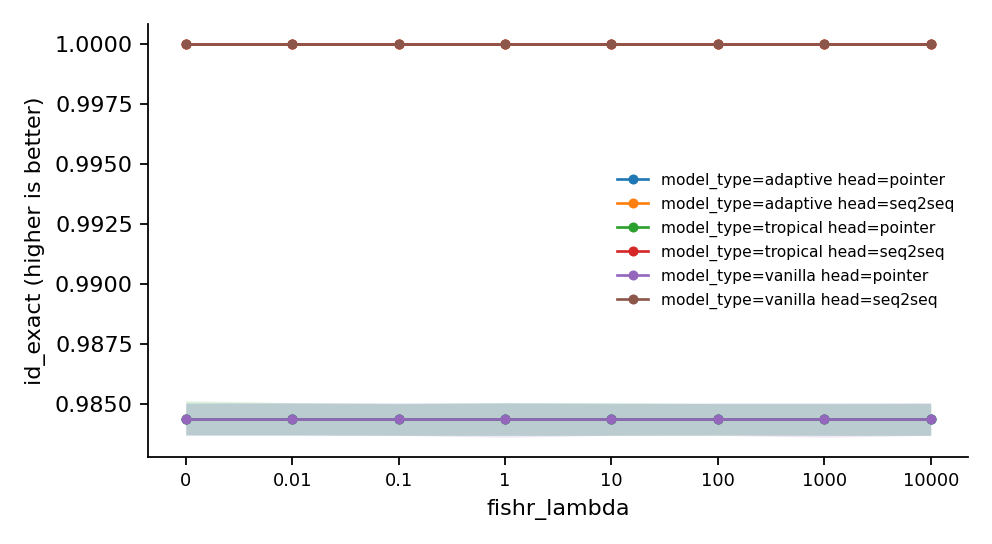
\includegraphics[width=\textwidth]{metric_id_exact.png}
\caption{\texttt{id\_exact} against \texttt{fishr\_lambda}: the mean over seeds with a 95\% bootstrap CI, one line per combination of the other factors.}
\label{fig:id_exact}
\end{figure}

{\small
\begin{longtable}{lllrlrrr}
\caption{\texttt{id\_exact} per cell: mean, 95\% bootstrap CI, SD, seeds, diverged runs.}\label{tab:summary-id_exact}\\
\toprule
\texttt{model\_type} & \texttt{head} & \texttt{fishr\_lambda} & mean & 95\% CI & SD & $n$ & div.\\
\midrule
\endhead
adaptive & pointer & 0 & 0.9844 & [0.984, 0.985] & $8.83\times10^{-4}$ & 5 & 0\\
adaptive & pointer & 0.01 & 0.9844 & [0.984, 0.985] & $8.83\times10^{-4}$ & 5 & 0\\
adaptive & pointer & 0.1 & 0.9844 & [0.984, 0.985] & $8.83\times10^{-4}$ & 5 & 0\\
adaptive & pointer & 1 & 0.9844 & [0.984, 0.985] & $8.83\times10^{-4}$ & 5 & 0\\
adaptive & pointer & 10 & 0.9844 & [0.984, 0.985] & $8.83\times10^{-4}$ & 5 & 0\\
adaptive & pointer & 100 & 0.9844 & [0.984, 0.985] & $8.83\times10^{-4}$ & 5 & 0\\
adaptive & pointer & 1000 & 0.9844 & [0.984, 0.985] & $8.83\times10^{-4}$ & 5 & 0\\
adaptive & pointer & 1e+04 & 0.9844 & [0.984, 0.985] & $8.83\times10^{-4}$ & 5 & 0\\
adaptive & seq2seq & 0 & 1 & [1, 1] & 0 & 5 & 0\\
adaptive & seq2seq & 0.01 & 1 & [1, 1] & 0 & 5 & 0\\
adaptive & seq2seq & 0.1 & 1 & [1, 1] & 0 & 5 & 0\\
adaptive & seq2seq & 1 & 1 & [1, 1] & 0 & 5 & 0\\
adaptive & seq2seq & 10 & 1 & [1, 1] & 0 & 5 & 0\\
adaptive & seq2seq & 100 & 1 & [1, 1] & 0 & 5 & 0\\
adaptive & seq2seq & 1000 & 1 & [1, 1] & 0 & 5 & 0\\
adaptive & seq2seq & 1e+04 & 1 & [1, 1] & 0 & 5 & 0\\
tropical & pointer & 0 & 0.9844 & [0.984, 0.985] & $8.83\times10^{-4}$ & 5 & 0\\
tropical & pointer & 0.01 & 0.9844 & [0.984, 0.985] & $8.83\times10^{-4}$ & 5 & 0\\
tropical & pointer & 0.1 & 0.9844 & [0.984, 0.985] & $8.83\times10^{-4}$ & 5 & 0\\
tropical & pointer & 1 & 0.9844 & [0.984, 0.985] & $8.83\times10^{-4}$ & 5 & 0\\
tropical & pointer & 10 & 0.9844 & [0.984, 0.985] & $8.83\times10^{-4}$ & 5 & 0\\
tropical & pointer & 100 & 0.9844 & [0.984, 0.985] & $8.83\times10^{-4}$ & 5 & 0\\
tropical & pointer & 1000 & 0.9844 & [0.984, 0.985] & $8.83\times10^{-4}$ & 5 & 0\\
tropical & pointer & 1e+04 & 0.9844 & [0.984, 0.985] & $8.83\times10^{-4}$ & 5 & 0\\
tropical & seq2seq & 0 & 1 & [1, 1] & 0 & 5 & 0\\
tropical & seq2seq & 0.01 & 1 & [1, 1] & 0 & 5 & 0\\
tropical & seq2seq & 0.1 & 1 & [1, 1] & 0 & 5 & 0\\
tropical & seq2seq & 1 & 1 & [1, 1] & 0 & 5 & 0\\
tropical & seq2seq & 10 & 1 & [1, 1] & 0 & 5 & 0\\
tropical & seq2seq & 100 & 1 & [1, 1] & 0 & 5 & 0\\
tropical & seq2seq & 1000 & 1 & [1, 1] & 0 & 5 & 0\\
tropical & seq2seq & 1e+04 & 1 & [1, 1] & 0 & 5 & 0\\
vanilla & pointer & 0 & 0.9844 & [0.984, 0.985] & $8.83\times10^{-4}$ & 5 & 0\\
vanilla & pointer & 0.01 & 0.9844 & [0.984, 0.985] & $8.83\times10^{-4}$ & 5 & 0\\
vanilla & pointer & 0.1 & 0.9844 & [0.984, 0.985] & $8.83\times10^{-4}$ & 5 & 0\\
vanilla & pointer & 1 & 0.9844 & [0.984, 0.985] & $8.83\times10^{-4}$ & 5 & 0\\
vanilla & pointer & 10 & 0.9844 & [0.984, 0.985] & $8.83\times10^{-4}$ & 5 & 0\\
vanilla & pointer & 100 & 0.9844 & [0.984, 0.985] & $8.83\times10^{-4}$ & 5 & 0\\
vanilla & pointer & 1000 & 0.9844 & [0.984, 0.985] & $8.83\times10^{-4}$ & 5 & 0\\
vanilla & pointer & 1e+04 & 0.9844 & [0.984, 0.985] & $8.83\times10^{-4}$ & 5 & 0\\
vanilla & seq2seq & 0 & 1 & [1, 1] & 0 & 5 & 0\\
vanilla & seq2seq & 0.01 & 1 & [1, 1] & 0 & 5 & 0\\
vanilla & seq2seq & 0.1 & 1 & [1, 1] & 0 & 5 & 0\\
vanilla & seq2seq & 1 & 1 & [1, 1] & 0 & 5 & 0\\
vanilla & seq2seq & 10 & 1 & [1, 1] & 0 & 5 & 0\\
vanilla & seq2seq & 100 & 1 & [1, 1] & 0 & 5 & 0\\
vanilla & seq2seq & 1000 & 1 & [1, 1] & 0 & 5 & 0\\
vanilla & seq2seq & 1e+04 & 1 & [1, 1] & 0 & 5 & 0\\
\bottomrule
\end{longtable}
}

{\small
\begin{longtable}{lllrrrl}
\caption{\texttt{id\_exact}: each level of \texttt{fishr\_lambda} against its control (0), within each combination of the other factors. rank: Wilcoxon signed-rank by seed, Holm.}\label{tab:control-id_exact}\\
\toprule
\texttt{model\_type} & \texttt{head} & \texttt{fishr\_lambda} & difference & 95\% CI & $p$ & \\
\midrule
\endhead
adaptive & pointer & 0.01 & 0 & [0, 0] & -- & \\
adaptive & pointer & 0.1 & 0 & [0, 0] & -- & \\
adaptive & pointer & 1 & 0 & [0, 0] & -- & \\
adaptive & pointer & 10 & 0 & [0, 0] & -- & \\
adaptive & pointer & 100 & 0 & [0, 0] & -- & \\
adaptive & pointer & 1000 & 0 & [0, 0] & -- & \\
adaptive & pointer & 1e+04 & 0 & [0, 0] & -- & \\
adaptive & seq2seq & 0.01 & 0 & [0, 0] & -- & \\
adaptive & seq2seq & 0.1 & 0 & [0, 0] & -- & \\
adaptive & seq2seq & 1 & 0 & [0, 0] & -- & \\
adaptive & seq2seq & 10 & 0 & [0, 0] & -- & \\
adaptive & seq2seq & 100 & 0 & [0, 0] & -- & \\
adaptive & seq2seq & 1000 & 0 & [0, 0] & -- & \\
adaptive & seq2seq & 1e+04 & 0 & [0, 0] & -- & \\
tropical & pointer & 0.01 & 0 & [0, 0] & -- & \\
tropical & pointer & 0.1 & 0 & [0, 0] & -- & \\
tropical & pointer & 1 & 0 & [0, 0] & -- & \\
tropical & pointer & 10 & 0 & [0, 0] & -- & \\
tropical & pointer & 100 & 0 & [0, 0] & -- & \\
tropical & pointer & 1000 & 0 & [0, 0] & -- & \\
tropical & pointer & 1e+04 & 0 & [0, 0] & -- & \\
tropical & seq2seq & 0.01 & 0 & [0, 0] & -- & \\
tropical & seq2seq & 0.1 & 0 & [0, 0] & -- & \\
tropical & seq2seq & 1 & 0 & [0, 0] & -- & \\
tropical & seq2seq & 10 & 0 & [0, 0] & -- & \\
tropical & seq2seq & 100 & 0 & [0, 0] & -- & \\
tropical & seq2seq & 1000 & 0 & [0, 0] & -- & \\
tropical & seq2seq & 1e+04 & 0 & [0, 0] & -- & \\
vanilla & pointer & 0.01 & 0 & [0, 0] & -- & \\
vanilla & pointer & 0.1 & 0 & [0, 0] & -- & \\
vanilla & pointer & 1 & 0 & [0, 0] & -- & \\
vanilla & pointer & 10 & 0 & [0, 0] & -- & \\
vanilla & pointer & 100 & 0 & [0, 0] & -- & \\
vanilla & pointer & 1000 & 0 & [0, 0] & -- & \\
vanilla & pointer & 1e+04 & 0 & [0, 0] & -- & \\
vanilla & seq2seq & 0.01 & 0 & [0, 0] & -- & \\
vanilla & seq2seq & 0.1 & 0 & [0, 0] & -- & \\
vanilla & seq2seq & 1 & 0 & [0, 0] & -- & \\
vanilla & seq2seq & 10 & 0 & [0, 0] & -- & \\
vanilla & seq2seq & 100 & 0 & [0, 0] & -- & \\
vanilla & seq2seq & 1000 & 0 & [0, 0] & -- & \\
vanilla & seq2seq & 1e+04 & 0 & [0, 0] & -- & \\
\bottomrule
\end{longtable}
}

{\small
\begin{longtable}{llrrrrr}
\caption{\texttt{id\_exact} against log10 \texttt{fishr\_lambda}: rank: Spearman rho, seed-bootstrap CI, with the Jonckheere--Terpstra ordered-trend $\tau$ and $p$.}\label{tab:trend-id_exact}\\
\toprule
\texttt{model\_type} & \texttt{head} & estimate & 95\% CI & $p$ & JT $\tau$ & JT $p$\\
\midrule
\endhead
adaptive & pointer & 0 & [0, 0] & 1.0000 & 0 & 1.0000\\
adaptive & seq2seq & -- & [--, --] & -- & -- & --\\
tropical & pointer & 0 & [0, 0] & 1.0000 & 0 & 1.0000\\
tropical & seq2seq & -- & [--, --] & -- & -- & --\\
vanilla & pointer & 0 & [0, 0] & 1.0000 & 0 & 1.0000\\
vanilla & seq2seq & -- & [--, --] & -- & -- & --\\
\bottomrule
\end{longtable}
}

{\small
\begin{longtable}{lrrrl}
\caption{\texttt{id\_exact}: paired contrasts by seed, Holm-corrected across the cells. rank: Wilcoxon signed-rank by seed, Holm.}\label{tab:paired-id_exact}\\
\toprule
contrast (within) & difference & 95\% CI & $p$ & \\
\midrule
\endhead
\stackcell{model\_type: tropical - vanilla\\\footnotesize head=pointer fishr\_lambda=0 } & 0 & [--, --] & -- & \\
\stackcell{model\_type: tropical - vanilla\\\footnotesize head=pointer fishr\_lambda=0.01 } & 0 & [--, --] & -- & \\
\stackcell{model\_type: tropical - vanilla\\\footnotesize head=pointer fishr\_lambda=0.1 } & 0 & [--, --] & -- & \\
\stackcell{model\_type: tropical - vanilla\\\footnotesize head=pointer fishr\_lambda=1 } & 0 & [--, --] & -- & \\
\stackcell{model\_type: tropical - vanilla\\\footnotesize head=pointer fishr\_lambda=10 } & 0 & [--, --] & -- & \\
\stackcell{model\_type: tropical - vanilla\\\footnotesize head=pointer fishr\_lambda=100 } & 0 & [--, --] & -- & \\
\stackcell{model\_type: tropical - vanilla\\\footnotesize head=pointer fishr\_lambda=1000 } & 0 & [--, --] & -- & \\
\stackcell{model\_type: tropical - vanilla\\\footnotesize head=pointer fishr\_lambda=1e+04 } & 0 & [--, --] & -- & \\
\stackcell{model\_type: tropical - vanilla\\\footnotesize head=seq2seq fishr\_lambda=0 } & 0 & [--, --] & -- & \\
\stackcell{model\_type: tropical - vanilla\\\footnotesize head=seq2seq fishr\_lambda=0.01 } & 0 & [--, --] & -- & \\
\stackcell{model\_type: tropical - vanilla\\\footnotesize head=seq2seq fishr\_lambda=0.1 } & 0 & [--, --] & -- & \\
\stackcell{model\_type: tropical - vanilla\\\footnotesize head=seq2seq fishr\_lambda=1 } & 0 & [--, --] & -- & \\
\stackcell{model\_type: tropical - vanilla\\\footnotesize head=seq2seq fishr\_lambda=10 } & 0 & [--, --] & -- & \\
\stackcell{model\_type: tropical - vanilla\\\footnotesize head=seq2seq fishr\_lambda=100 } & 0 & [--, --] & -- & \\
\stackcell{model\_type: tropical - vanilla\\\footnotesize head=seq2seq fishr\_lambda=1000 } & 0 & [--, --] & -- & \\
\stackcell{model\_type: tropical - vanilla\\\footnotesize head=seq2seq fishr\_lambda=1e+04 } & 0 & [--, --] & -- & \\
\stackcell{model\_type: adaptive - vanilla\\\footnotesize head=pointer fishr\_lambda=0 } & 0 & [--, --] & -- & \\
\stackcell{model\_type: adaptive - vanilla\\\footnotesize head=pointer fishr\_lambda=0.01 } & 0 & [--, --] & -- & \\
\stackcell{model\_type: adaptive - vanilla\\\footnotesize head=pointer fishr\_lambda=0.1 } & 0 & [--, --] & -- & \\
\stackcell{model\_type: adaptive - vanilla\\\footnotesize head=pointer fishr\_lambda=1 } & 0 & [--, --] & -- & \\
\stackcell{model\_type: adaptive - vanilla\\\footnotesize head=pointer fishr\_lambda=10 } & 0 & [--, --] & -- & \\
\stackcell{model\_type: adaptive - vanilla\\\footnotesize head=pointer fishr\_lambda=100 } & 0 & [--, --] & -- & \\
\stackcell{model\_type: adaptive - vanilla\\\footnotesize head=pointer fishr\_lambda=1000 } & 0 & [--, --] & -- & \\
\stackcell{model\_type: adaptive - vanilla\\\footnotesize head=pointer fishr\_lambda=1e+04 } & 0 & [--, --] & -- & \\
\stackcell{model\_type: adaptive - vanilla\\\footnotesize head=seq2seq fishr\_lambda=0 } & 0 & [--, --] & -- & \\
\stackcell{model\_type: adaptive - vanilla\\\footnotesize head=seq2seq fishr\_lambda=0.01 } & 0 & [--, --] & -- & \\
\stackcell{model\_type: adaptive - vanilla\\\footnotesize head=seq2seq fishr\_lambda=0.1 } & 0 & [--, --] & -- & \\
\stackcell{model\_type: adaptive - vanilla\\\footnotesize head=seq2seq fishr\_lambda=1 } & 0 & [--, --] & -- & \\
\stackcell{model\_type: adaptive - vanilla\\\footnotesize head=seq2seq fishr\_lambda=10 } & 0 & [--, --] & -- & \\
\stackcell{model\_type: adaptive - vanilla\\\footnotesize head=seq2seq fishr\_lambda=100 } & 0 & [--, --] & -- & \\
\stackcell{model\_type: adaptive - vanilla\\\footnotesize head=seq2seq fishr\_lambda=1000 } & 0 & [--, --] & -- & \\
\stackcell{model\_type: adaptive - vanilla\\\footnotesize head=seq2seq fishr\_lambda=1e+04 } & 0 & [--, --] & -- & \\
\stackcell{head: pointer - seq2seq\\\footnotesize model\_type=adaptive fishr\_lambda=0 } & -0.0156 & [-0.0167, -0.0145] & 1.0000 & \\
\stackcell{head: pointer - seq2seq\\\footnotesize model\_type=adaptive fishr\_lambda=0.01 } & -0.0156 & [-0.0167, -0.0145] & 1.0000 & \\
\stackcell{head: pointer - seq2seq\\\footnotesize model\_type=adaptive fishr\_lambda=0.1 } & -0.0156 & [-0.0167, -0.0145] & 1.0000 & \\
\stackcell{head: pointer - seq2seq\\\footnotesize model\_type=adaptive fishr\_lambda=1 } & -0.0156 & [-0.0167, -0.0145] & 1.0000 & \\
\stackcell{head: pointer - seq2seq\\\footnotesize model\_type=adaptive fishr\_lambda=10 } & -0.0156 & [-0.0167, -0.0145] & 1.0000 & \\
\stackcell{head: pointer - seq2seq\\\footnotesize model\_type=adaptive fishr\_lambda=100 } & -0.0156 & [-0.0167, -0.0145] & 1.0000 & \\
\stackcell{head: pointer - seq2seq\\\footnotesize model\_type=adaptive fishr\_lambda=1000 } & -0.0156 & [-0.0167, -0.0145] & 1.0000 & \\
\stackcell{head: pointer - seq2seq\\\footnotesize model\_type=adaptive fishr\_lambda=1e+04 } & -0.0156 & [-0.0167, -0.0145] & 1.0000 & \\
\stackcell{head: pointer - seq2seq\\\footnotesize model\_type=tropical fishr\_lambda=0 } & -0.0156 & [-0.0167, -0.0145] & 1.0000 & \\
\stackcell{head: pointer - seq2seq\\\footnotesize model\_type=tropical fishr\_lambda=0.01 } & -0.0156 & [-0.0167, -0.0145] & 1.0000 & \\
\stackcell{head: pointer - seq2seq\\\footnotesize model\_type=tropical fishr\_lambda=0.1 } & -0.0156 & [-0.0167, -0.0145] & 1.0000 & \\
\stackcell{head: pointer - seq2seq\\\footnotesize model\_type=tropical fishr\_lambda=1 } & -0.0156 & [-0.0167, -0.0145] & 1.0000 & \\
\stackcell{head: pointer - seq2seq\\\footnotesize model\_type=tropical fishr\_lambda=10 } & -0.0156 & [-0.0167, -0.0145] & 1.0000 & \\
\stackcell{head: pointer - seq2seq\\\footnotesize model\_type=tropical fishr\_lambda=100 } & -0.0156 & [-0.0167, -0.0145] & 1.0000 & \\
\stackcell{head: pointer - seq2seq\\\footnotesize model\_type=tropical fishr\_lambda=1000 } & -0.0156 & [-0.0167, -0.0145] & 1.0000 & \\
\stackcell{head: pointer - seq2seq\\\footnotesize model\_type=tropical fishr\_lambda=1e+04 } & -0.0156 & [-0.0167, -0.0145] & 1.0000 & \\
\stackcell{head: pointer - seq2seq\\\footnotesize model\_type=vanilla fishr\_lambda=0 } & -0.0156 & [-0.0167, -0.0145] & 1.0000 & \\
\stackcell{head: pointer - seq2seq\\\footnotesize model\_type=vanilla fishr\_lambda=0.01 } & -0.0156 & [-0.0167, -0.0145] & 1.0000 & \\
\stackcell{head: pointer - seq2seq\\\footnotesize model\_type=vanilla fishr\_lambda=0.1 } & -0.0156 & [-0.0167, -0.0145] & 1.0000 & \\
\stackcell{head: pointer - seq2seq\\\footnotesize model\_type=vanilla fishr\_lambda=1 } & -0.0156 & [-0.0167, -0.0145] & 1.0000 & \\
\stackcell{head: pointer - seq2seq\\\footnotesize model\_type=vanilla fishr\_lambda=10 } & -0.0156 & [-0.0167, -0.0145] & 1.0000 & \\
\stackcell{head: pointer - seq2seq\\\footnotesize model\_type=vanilla fishr\_lambda=100 } & -0.0156 & [-0.0167, -0.0145] & 1.0000 & \\
\stackcell{head: pointer - seq2seq\\\footnotesize model\_type=vanilla fishr\_lambda=1000 } & -0.0156 & [-0.0167, -0.0145] & 1.0000 & \\
\stackcell{head: pointer - seq2seq\\\footnotesize model\_type=vanilla fishr\_lambda=1e+04 } & -0.0156 & [-0.0167, -0.0145] & 1.0000 & \\
\bottomrule
\end{longtable}
}


\section{Curves}
\begin{figure}[tbp]
\centering
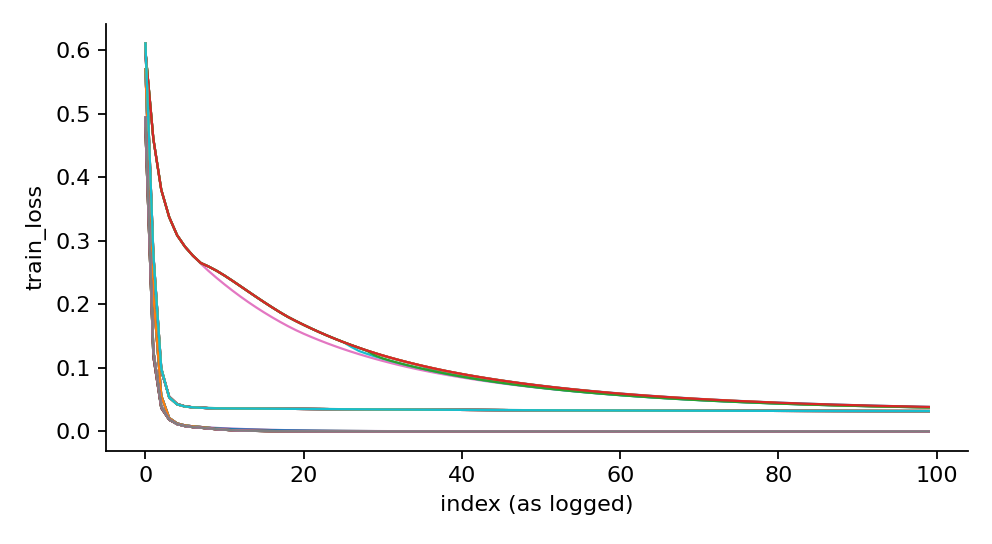
\includegraphics[width=\textwidth]{curve_train_loss.png}
\caption{\texttt{train\_loss}, the mean over seeds per cell.}
\label{fig:curve-1}
\end{figure}
\begin{figure}[tbp]
\centering
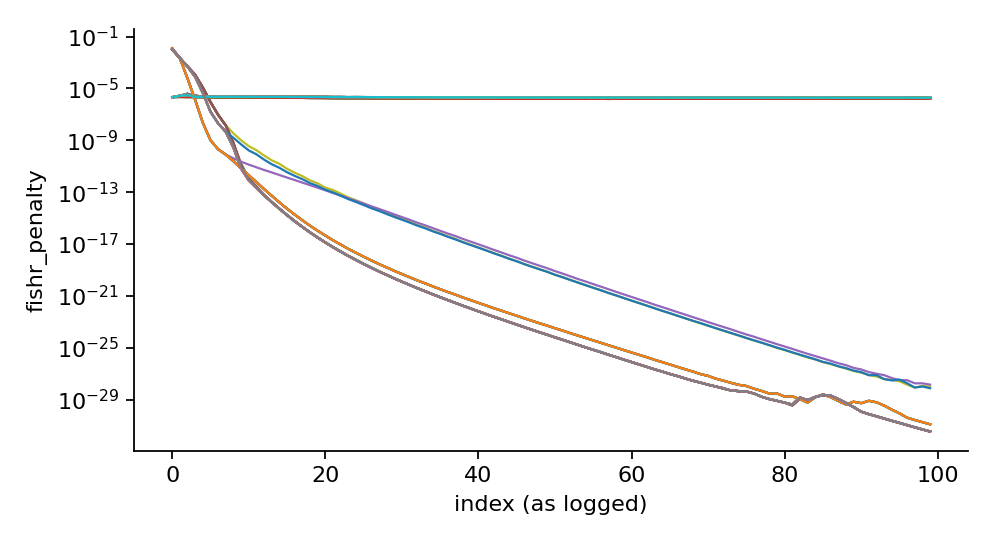
\includegraphics[width=\textwidth]{curve_fishr_penalty.png}
\caption{\texttt{fishr\_penalty}, the mean over seeds per cell.}
\label{fig:curve-2}
\end{figure}
\begin{figure}[tbp]
\centering
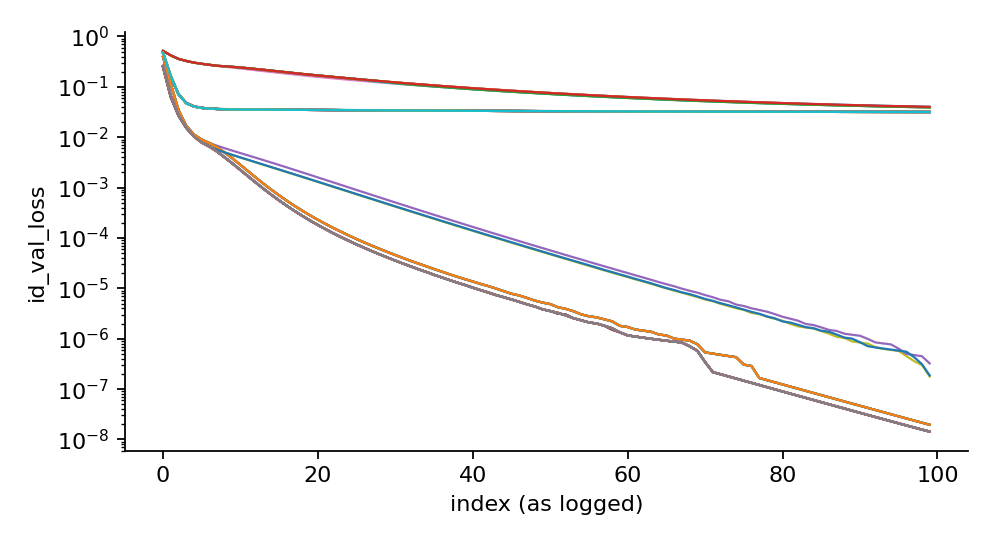
\includegraphics[width=\textwidth]{curve_id_val_loss.png}
\caption{\texttt{id\_val\_loss}, the mean over seeds per cell.}
\label{fig:curve-3}
\end{figure}

\section{Configuration}
The base configuration every run shares (frozen hash \texttt{ff2962d32940}); factor levels are in \autoref{tab:summary-ood_len_f1}.
{\footnotesize
\begin{verbatim}
task:
  name: MaxSubsetSumDataset
  value_range:
  - -5
  - 5
  target_range: null
  weight_range: null
  adversarial_range:
  - 10
  - 30
  noise_prob: 0.0
data:
  train_lengths:
  - 4
  - 5
  - 6
  - 7
  - 8
  ood_lengths:
  - 12
  - 16
  - 64
  ood_value_range: null
  ood_noise_range: null
  ood_noise_prob: 0.5
  n_per_length: 20000
  n_eval_per_length: 2000
  curve_eval_limit: 256
model:
  d_model: 64
  n_heads: 2
  num_layers: 1
  dropout: 0.0
  tropical_impl: legacy
optim:
  lr: 0.0001
  epochs: 100
  batch_size: 100
  eval_batch_size: 256
fishr:
  ema: 0.95
  anneal_iters: 1500
  reset_optimizer: true
\end{verbatim}
}
Store: \texttt{campaigns/tropical/MaxSubsetSum/results}.
\end{document}